\chapter{Viability of our Approach}
\label{sec:SEC}

As mentioned earlier, the viability of this approach was tested in~\cite{kechengthesis}. 
They used a pipelining algorithm to generate a pipeline reference model and compared their pipelined 
implementation with pipelined RTL using SEC to justify their approach. 

If we replace their algorithm with our certified algorithm and still produce the same pipelined implementation with same shadow registers and data propagations, we can claim that our algorithm is also suited for certifying behaviorally synthesized designs. 

\section{Experimental Results}

We ran our algorithm on industrial strength pipelined designs synthesized by AutoESL (c.f Figure~\ref{fig:testing}). 


\begin{figure}[h]
\begin{center}
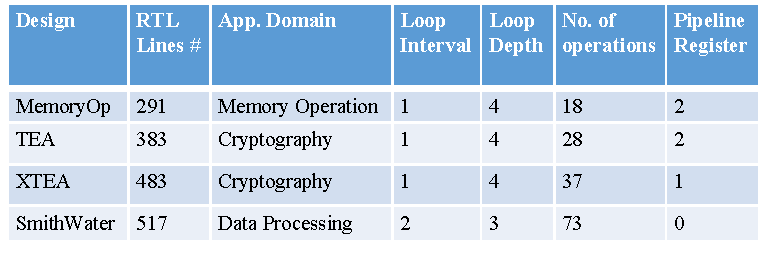
\includegraphics[width=5.5in]{fig-proposal/testing}
\end{center}
\caption{Behaviorally synthesized pipelined designs tested using our algorithm}
\label{fig:testing}
\end{figure}


We have successfully tested the pipeline reference model generated by our certified algorithm with the pipelined reference model generated by the previous algorithm. The test designs are non-trivial to pipeline with varied pipeline intervals and depths and require data forwarding and use of temporary shadow registers to remove data hazards. 

\section{Walk Through Of Our Approach For An Industrial Strength Design}

To understand our approach, we can go over the steps of one particular industrial strength design.

\begin{figure}[H]
\begin{center}
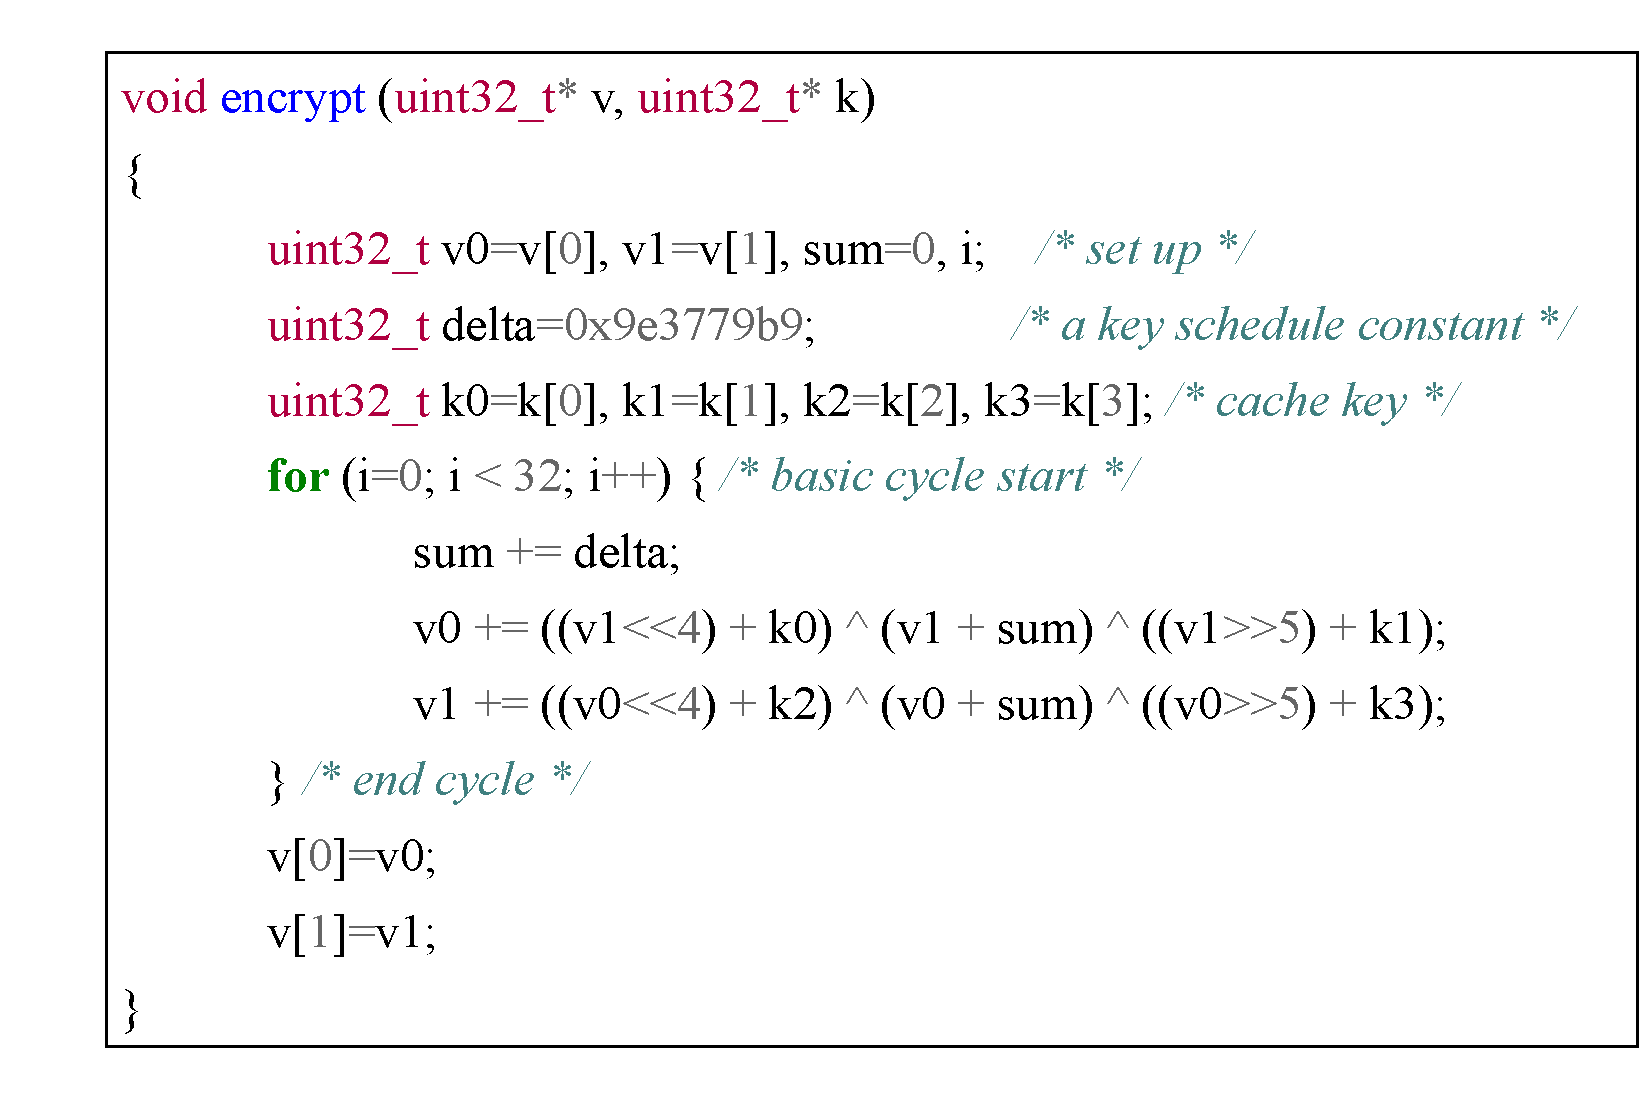
\includegraphics[width=5.5in]{fig-proposal/C-code-tea}
\end{center}
\caption{TEA: C code}
\label{fig:C-code-tea}
\end{figure}

Tiny Encryption Algorithm (TEA)~\cite{book-tea1} is a cryptography design. It is a block cipher notable for its simplicity of description and implementation with a few lines of code as shown in Figure~\ref{fig:C-code-tea}. TEA operates on two 32-bit unsigned integers (could be derived from a 64-bit data block) and uses a 128-bit key.  It has a simple key usage, mixing all of the key material in exactly the same way for each cycle. Different multiples of a magic constant are used to prevent simple attacks based on the symmetry of the rounds. The magic constant, 2654435769 or 9E3779B916 is chosen to be 232/$\phi$, where $\phi$ is the golden ratio''.  

The C code is converted to an Intermediate representation $IR$ and undergoes compiler transformations. If we only consider the loop CCDFG, ignoring the paraphernalia before and after this, we have a loop sequential CCDFG just before the loop pipelining transformtion needs to be applied as shown in Figure~\ref{fig:tea-seq-loop-ccdfg}. Now, we show how we apply our algorithm to derive a pipelined loop structure from this sequential CCDFG. 

Recall that the first step of the algorithm is to remove branches. Assuming that the loop exits in the (k + 1)st iteration, we separate $S_{loop}$ and $S_{preExit}$ as we explained earlier in Chapter 5. We now have a CCDFG as shown in Figure~\ref{fig:tea-algorithm-after-removing-branches}.

Next, we unroll the loop once to separate the first iteration from the rest. Recall that this step is important so that we can statically determine how to resolve the 
$\phi$-construct. The unrolled loop structure is shown in Figure~\ref{fig:tea-algorithm-two-iterations}.

Next, we resolve the $\phi$-construct and replace it with appropriate assignment statements as explained in $\phi$-removal step in Chapter 5. Note that the
first iteration of the loop has the previous basic block as $Entry$ so $\phi$-construct resolution is different than those in other iterations where previous basic block is $Z$. The CCDFG after this step is as shown in Figure~\ref{fig:tea-after-phi-removal}.

\begin{figure}[H]
\begin{center}
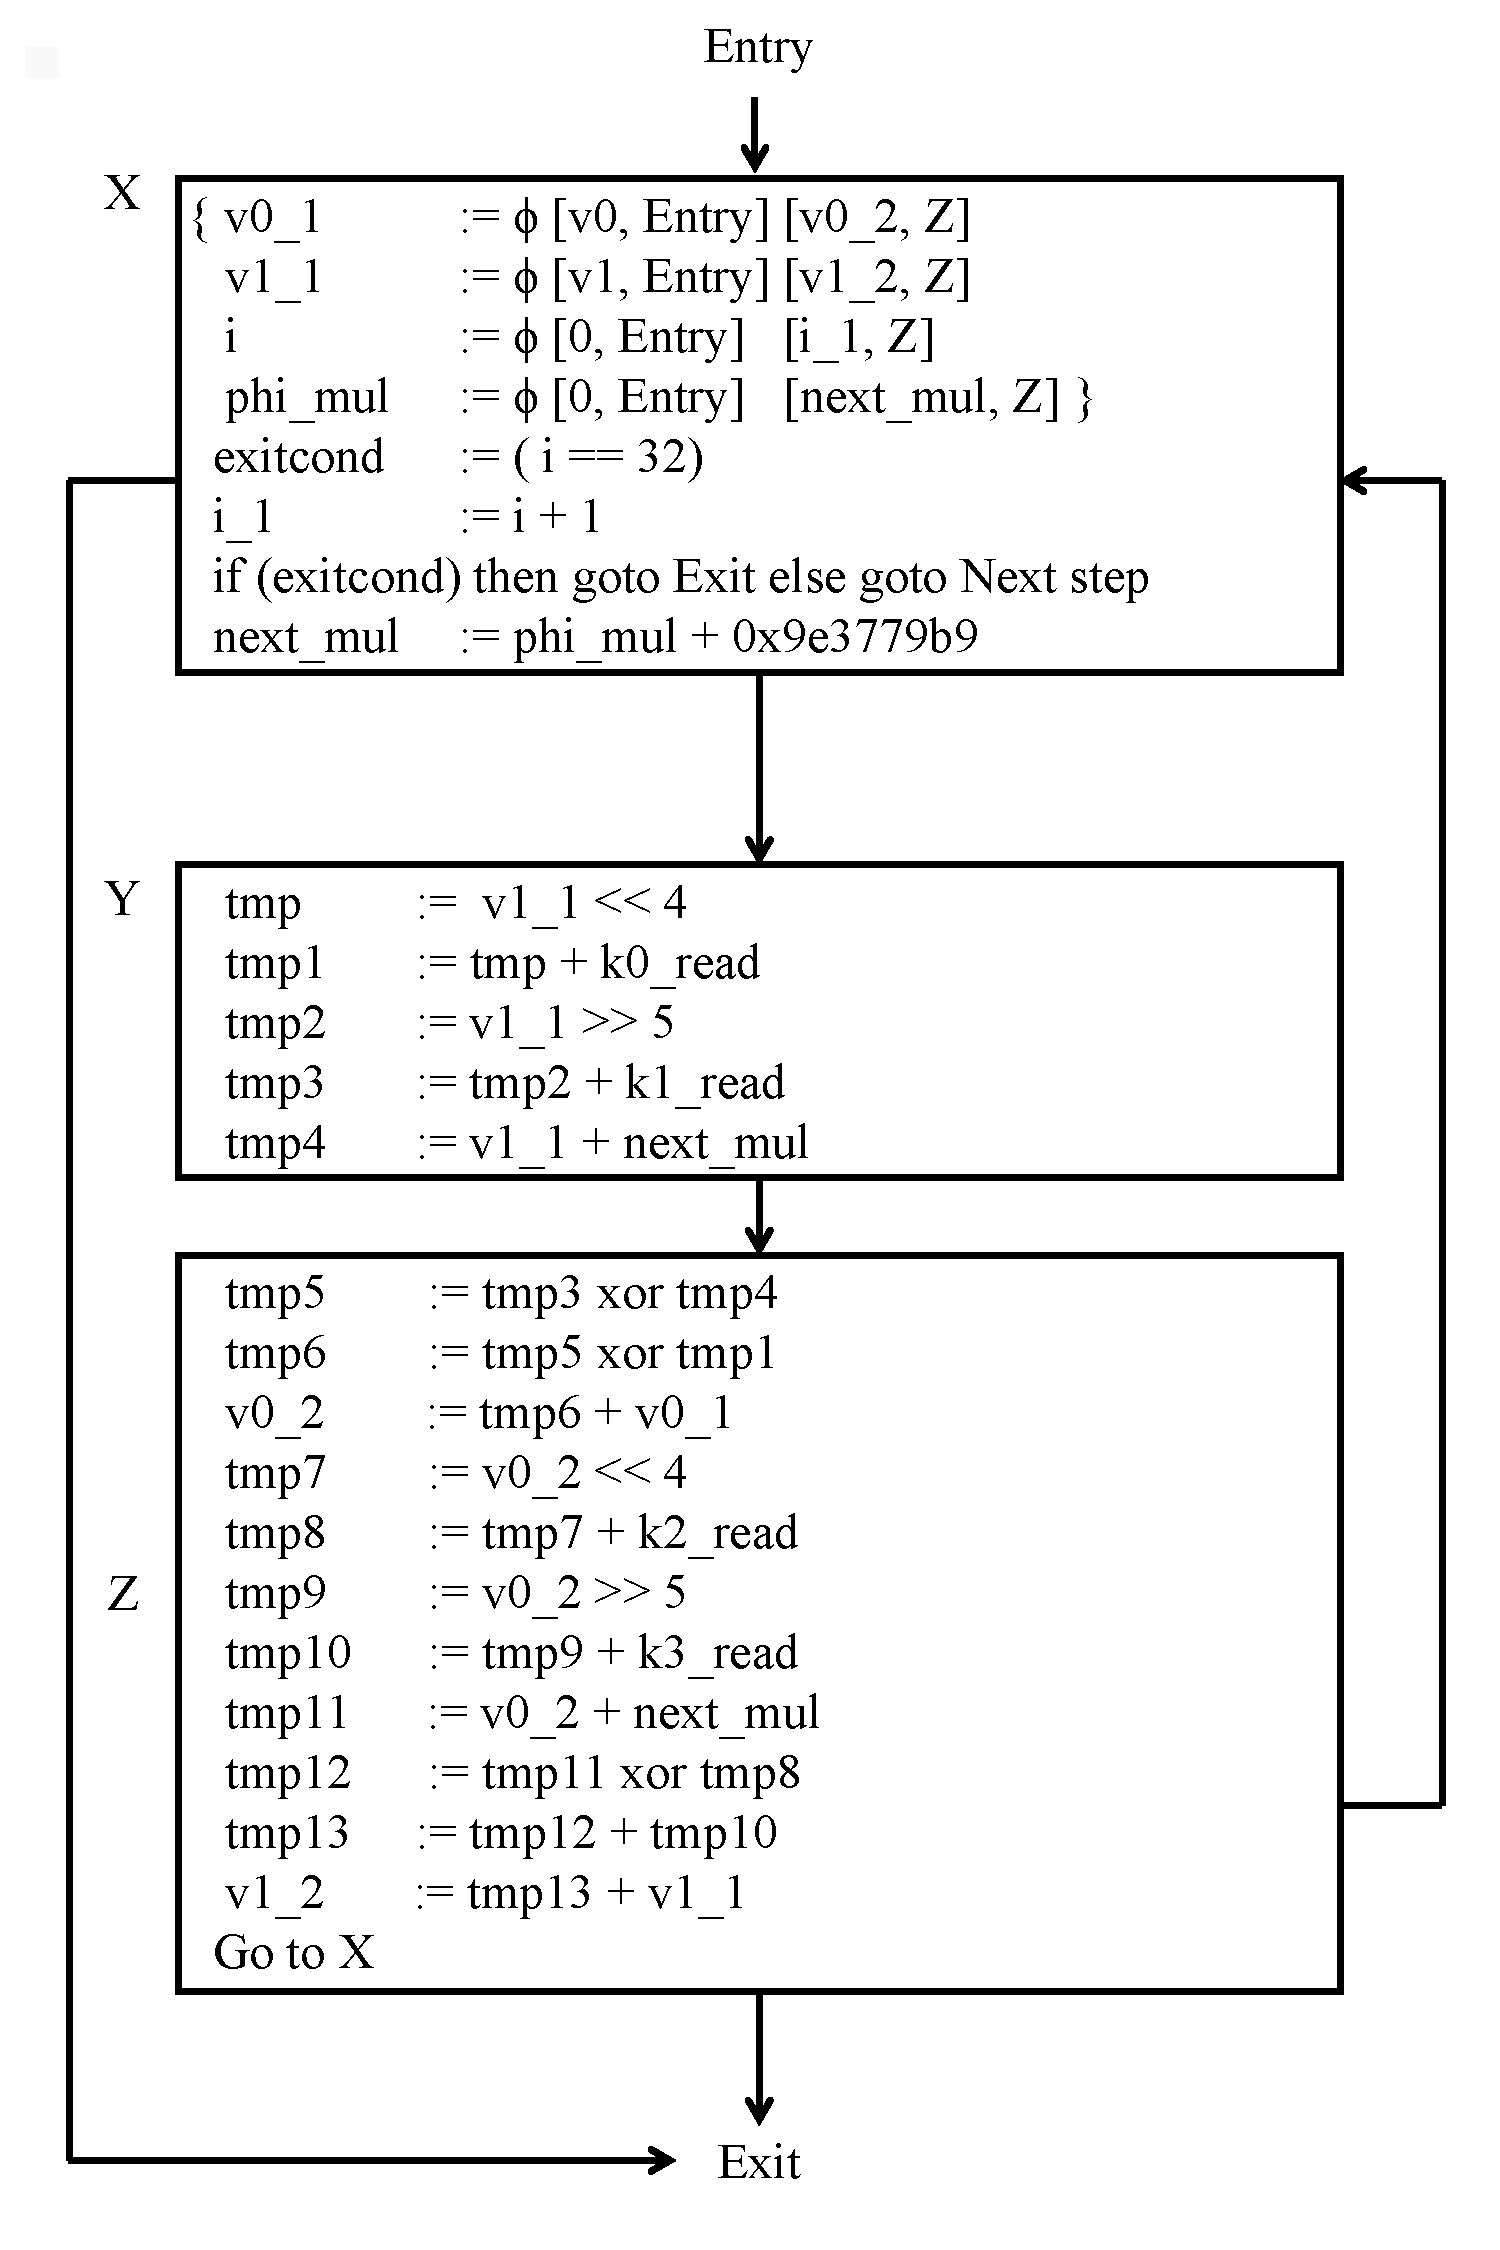
\includegraphics[width=4.75in]{fig-proposal/tea-seq-ccdfg}
\caption{TEA: Sequential Loop CCDFG}
\label{fig:tea-seq-loop-ccdfg}
\end{center}
\end{figure}

\begin{figure}[H]
\begin{center}
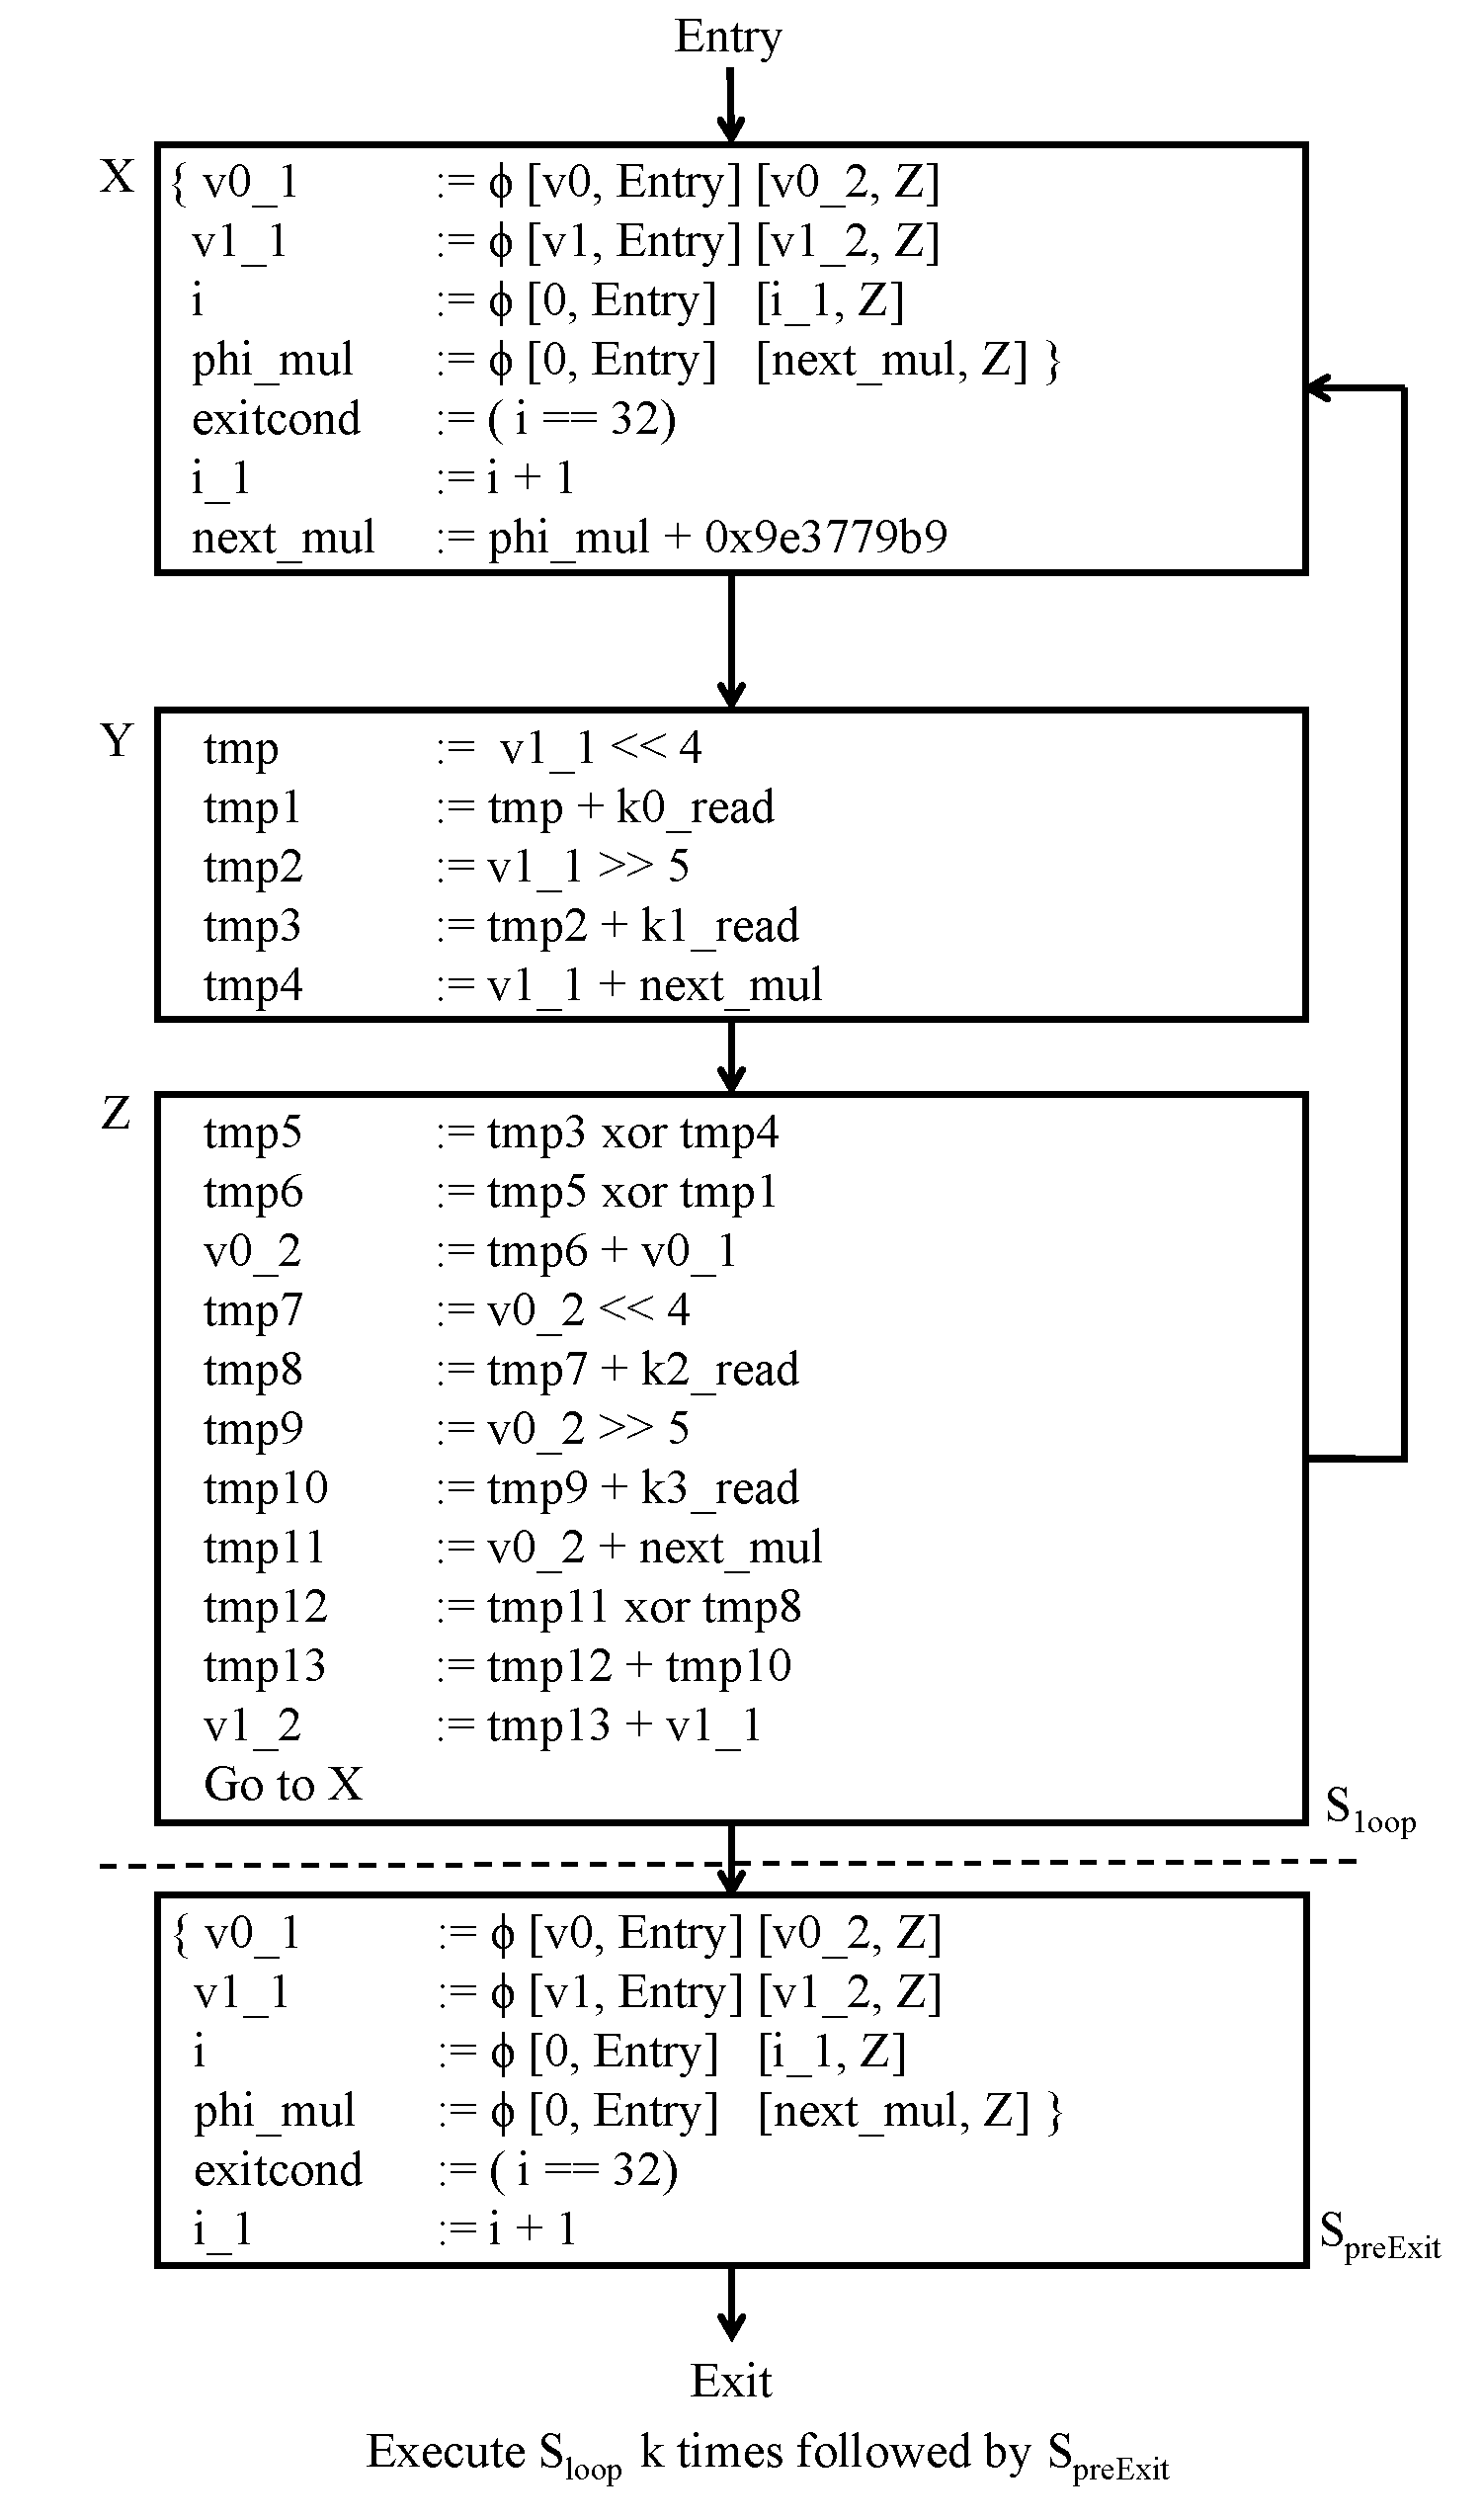
\includegraphics[height=8in]{fig-proposal/tea-algorithm-after-removing-branches}
\caption{TEA: After Removing Branches}
\label{fig:tea-algorithm-after-removing-branches}
\end{center}
\end{figure}

\begin{figure}[H]
\begin{center}
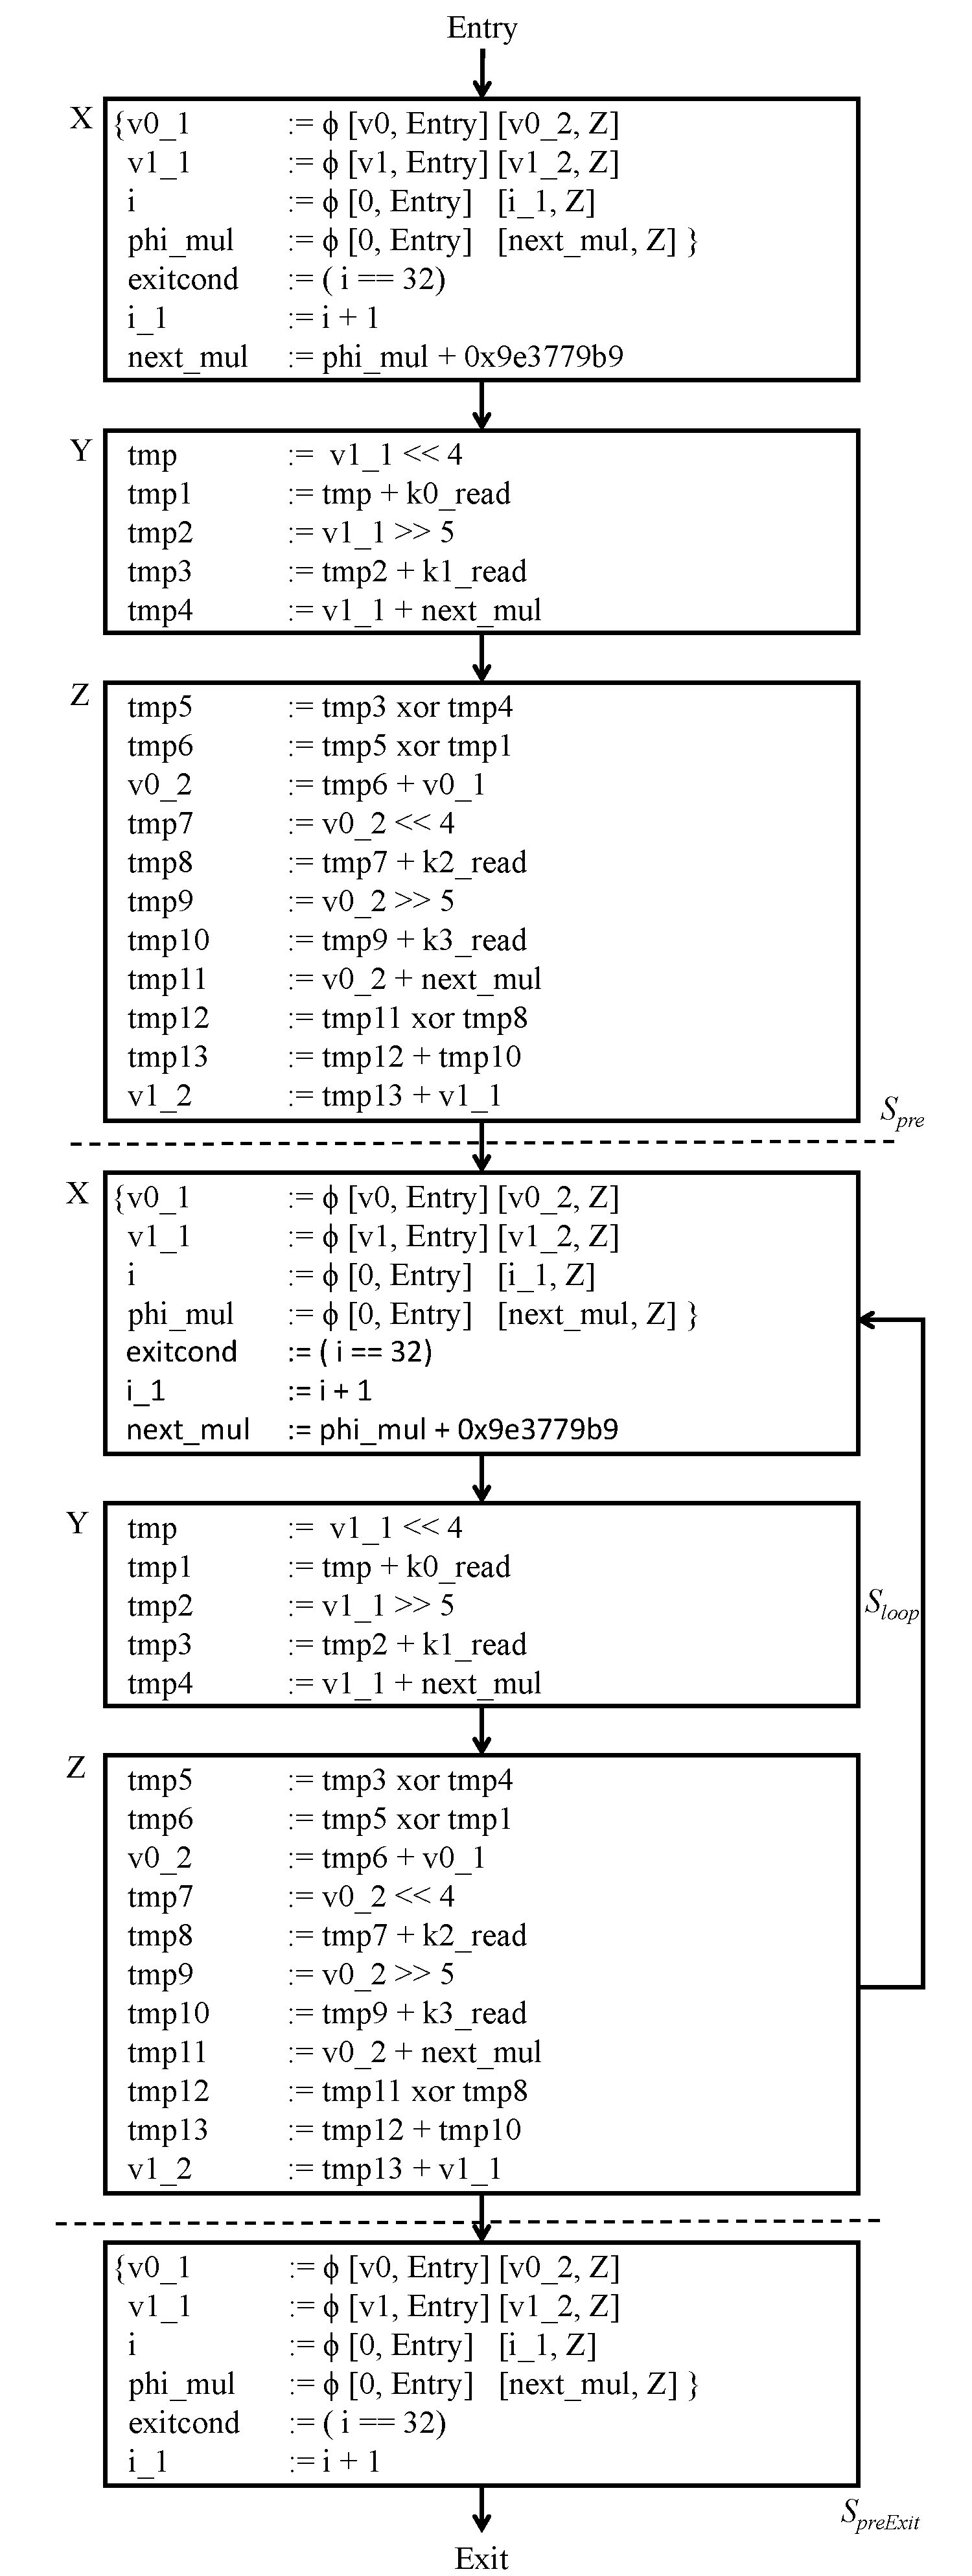
\includegraphics[height=8in]{fig-proposal/tea-after-two-iterations}
\caption{TEA: After Unrolling Loop Once}
\label{fig:tea-algorithm-two-iterations}
\end{center}
\end{figure}


\begin{figure}[H]
\begin{center}
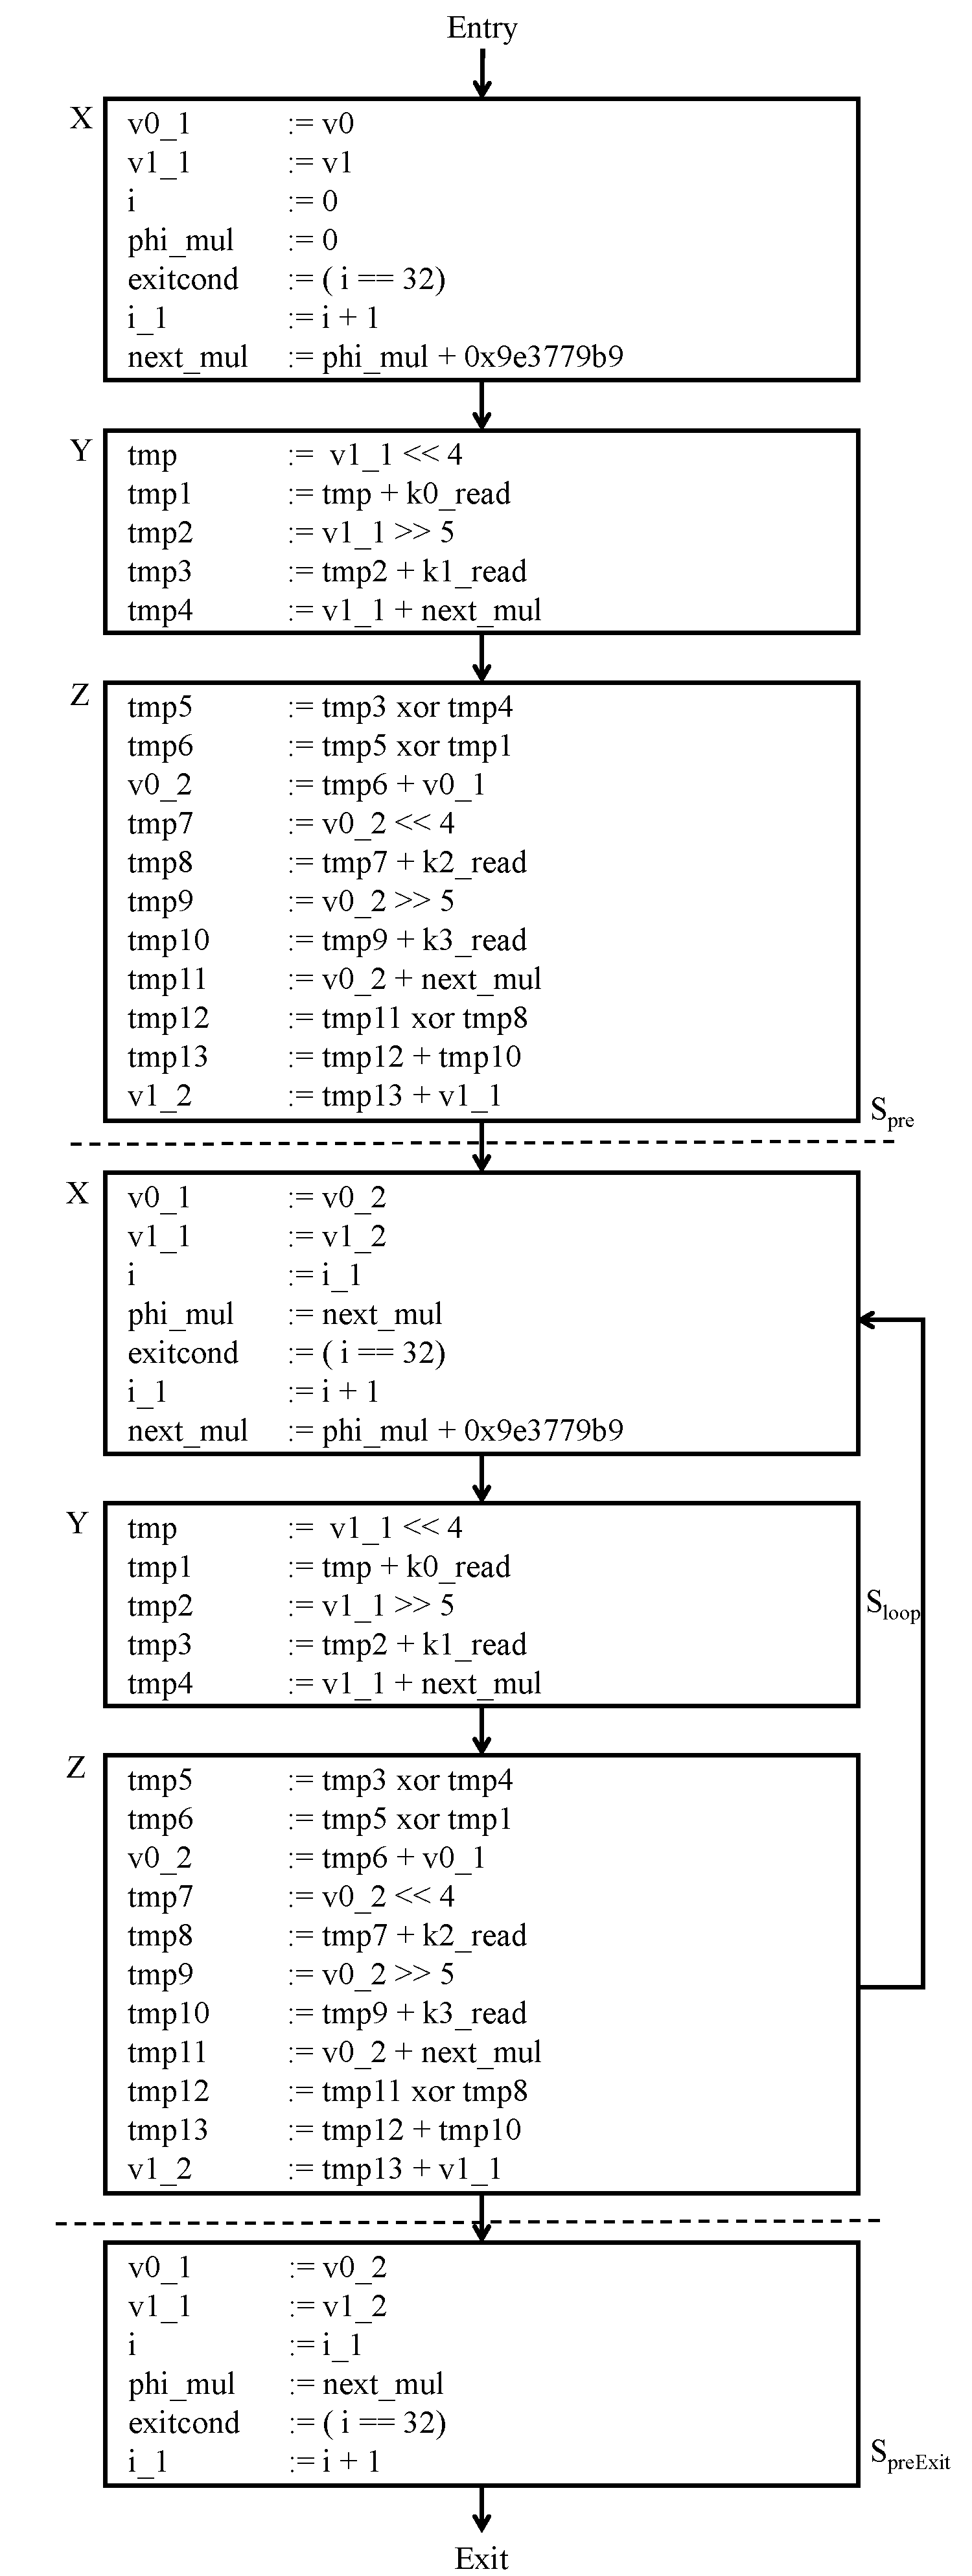
\includegraphics[height=8in]{fig-proposal/tea-after-phi-removal}
\caption{TEA: After $\phi$-removal}
\label{fig:tea-after-phi-removal}
\end{center}
\end{figure}

Now, we have to prepare this CCDFG so that iterations can be overlapped. So, we need to remove the data hazards. We first identify the variables/microsteps which 
cause Write After Read (WAR) hazards. We note that values of v0\_1 and v1\_1 are read in $X$ and written in $Z$ of $S_{loop}$. If we overlap the iterations, then $X$ of second iteration will read the outdated values of these variables before they have had a chance to be updated by the $Z$ of the first iteration, thus causing data hazards. 

To overcome this, recall that we have data propagation step in Chapter 5 as next step of our algorithm. We implement the first step for $v0\_1 := v0\_2$ 
and move it to the beginning of the X block in $S_{loop}$ and $S_{preExit}$ as shown in Figure~\ref{fig:tea-after-data-propagation1}. Since, we are already at the beginning of $S_{loop}$ here, nothing needs to be done. Recall, this step may need multiple applictions of interchange primitive. 

In the second step, we add this microstep to $Z$ of $S_{pre}$ and $Z$ of $S_{loop}$ and remove this mstep from $X$ of $S_{loop}$ and $X$ of $S_{preExit}$ as shown in Figure~\ref{fig:tea-after-data-propagation2}. The motivation is to move the microstep to the previous iteration such that the value of any variable is overwritten only when the previous value has already been correctly read. The justification of this step is as explained in Chapter 6 using smart restructing of CCDFG to ease the complexity and application of multiple interchange primitives. 

We apply both the steps of data propagation primitive for the second mstep as well, as shown $v1\_1 := v1\_2$ in Figures~\ref{fig:tea-after-data-propagation3} and~\ref{fig:tea-after-data-propagation4}.

\begin{figure}[H]
\begin{center}
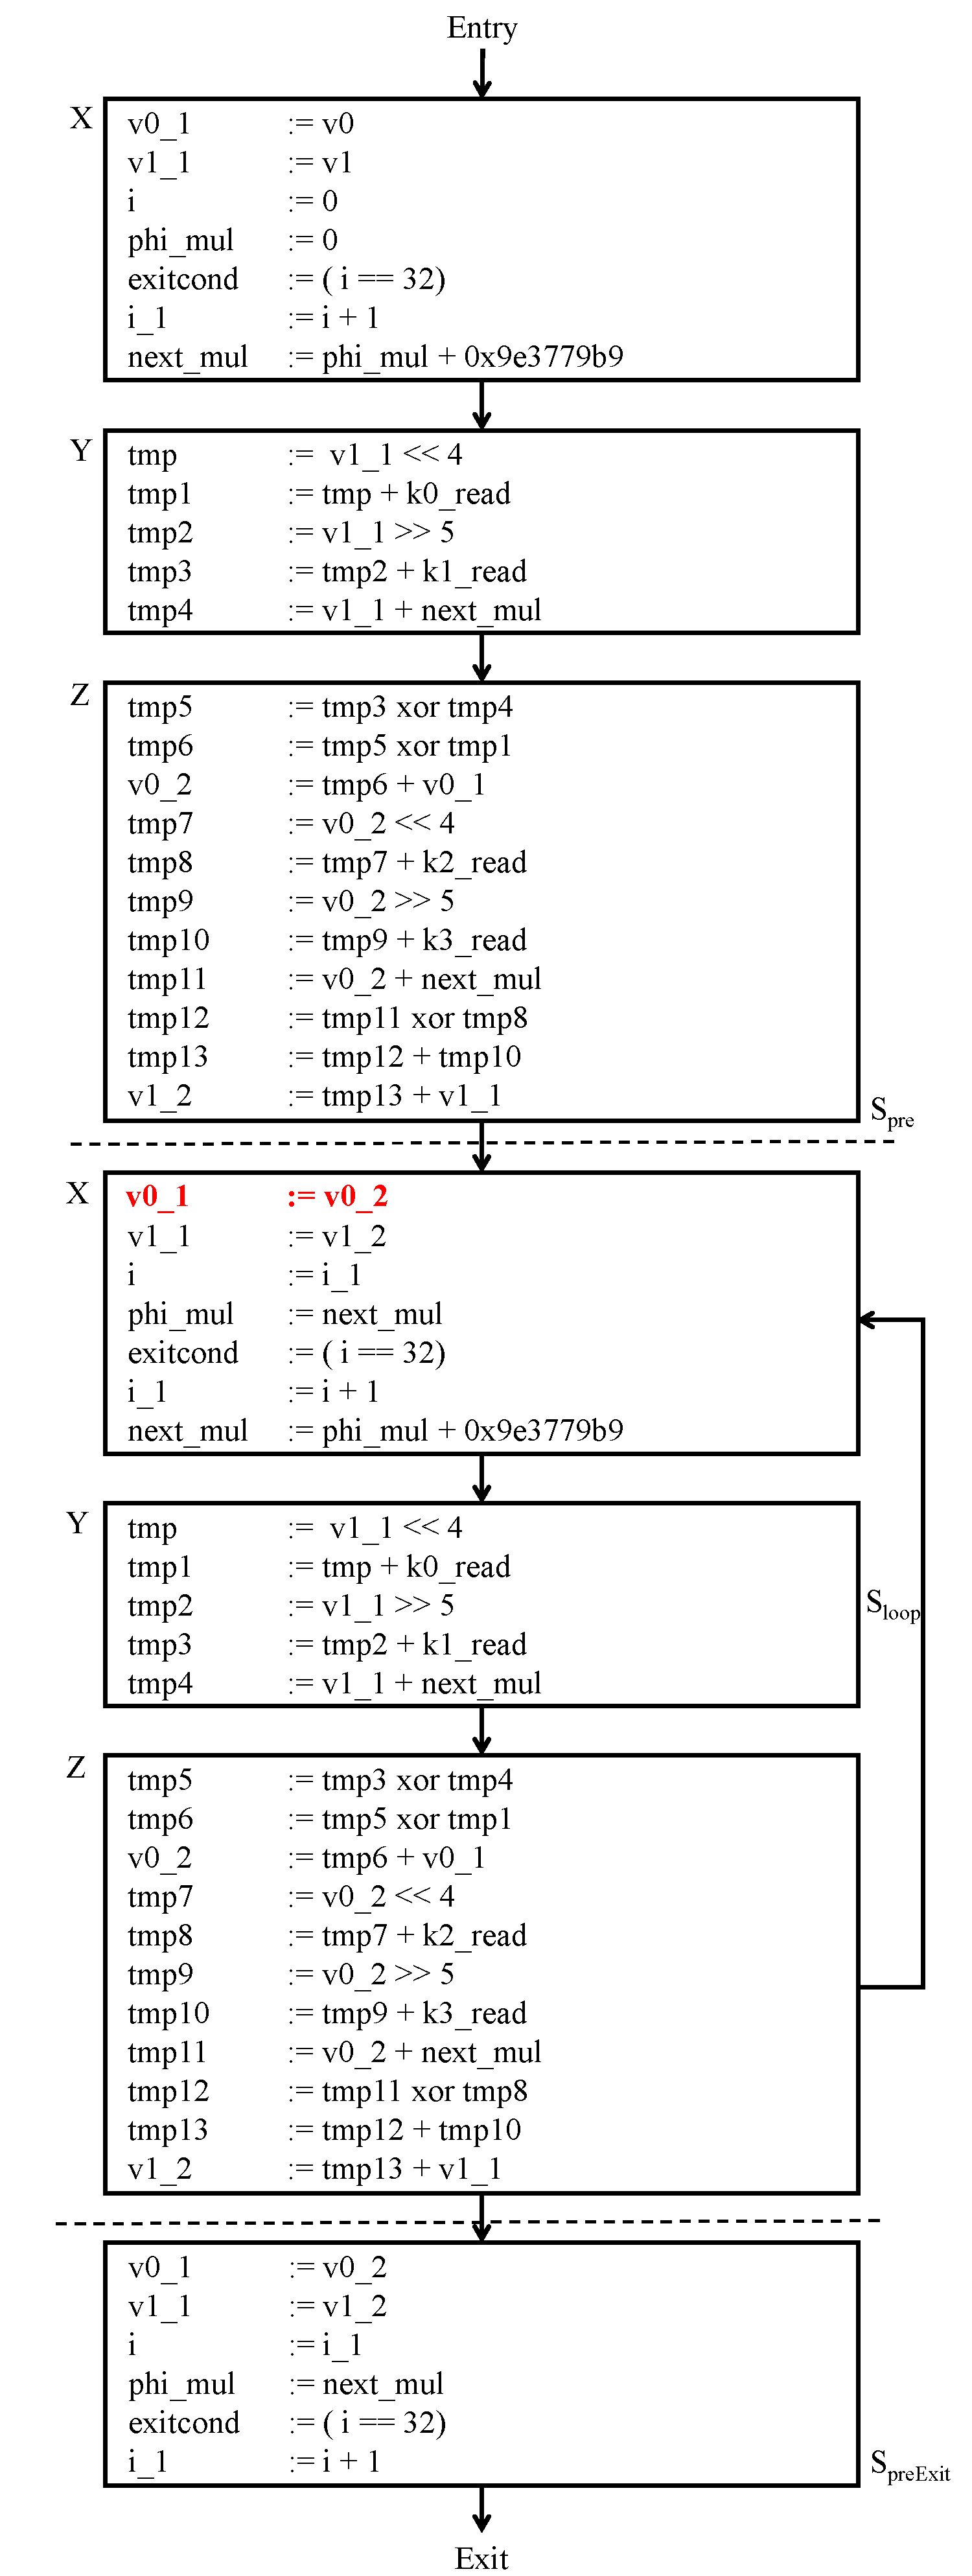
\includegraphics[height=8in]{fig-proposal/tea-after-data-propagation1}
\caption{TEA: After Data Propagation First Step for $v0\_1 := v0\_2$}
\label{fig:tea-after-data-propagation1}
\end{center}
\end{figure}

\begin{figure}[H]
\begin{center}
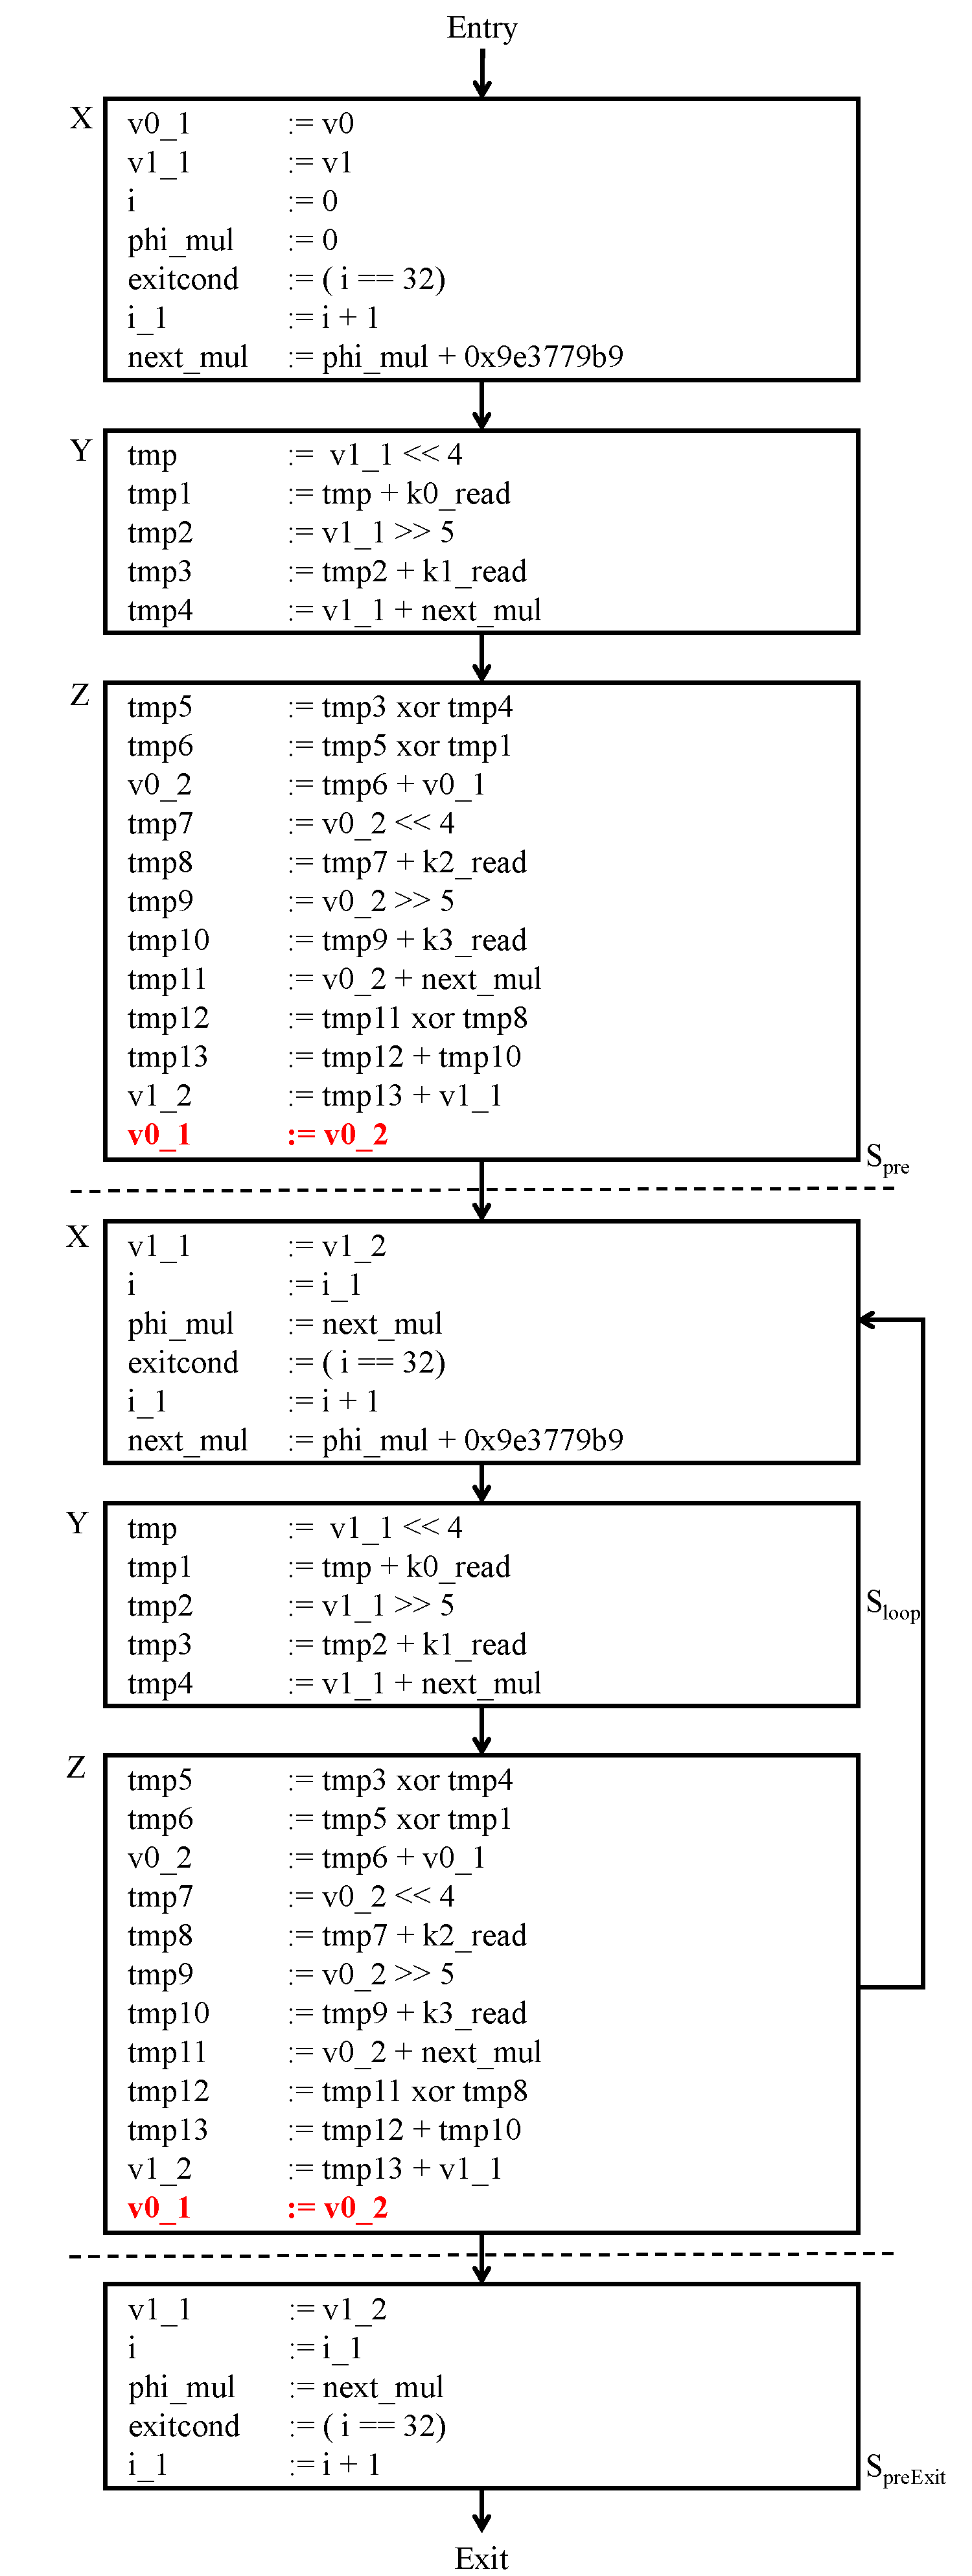
\includegraphics[height=8in]{fig-proposal/tea-after-data-propagation2}
\caption{TEA: After Data Propagation Second Step for $v0\_1 := v0\_2$}
\label{fig:tea-after-data-propagation2}
\end{center}
\end{figure}

\begin{figure}[H]
\begin{center}
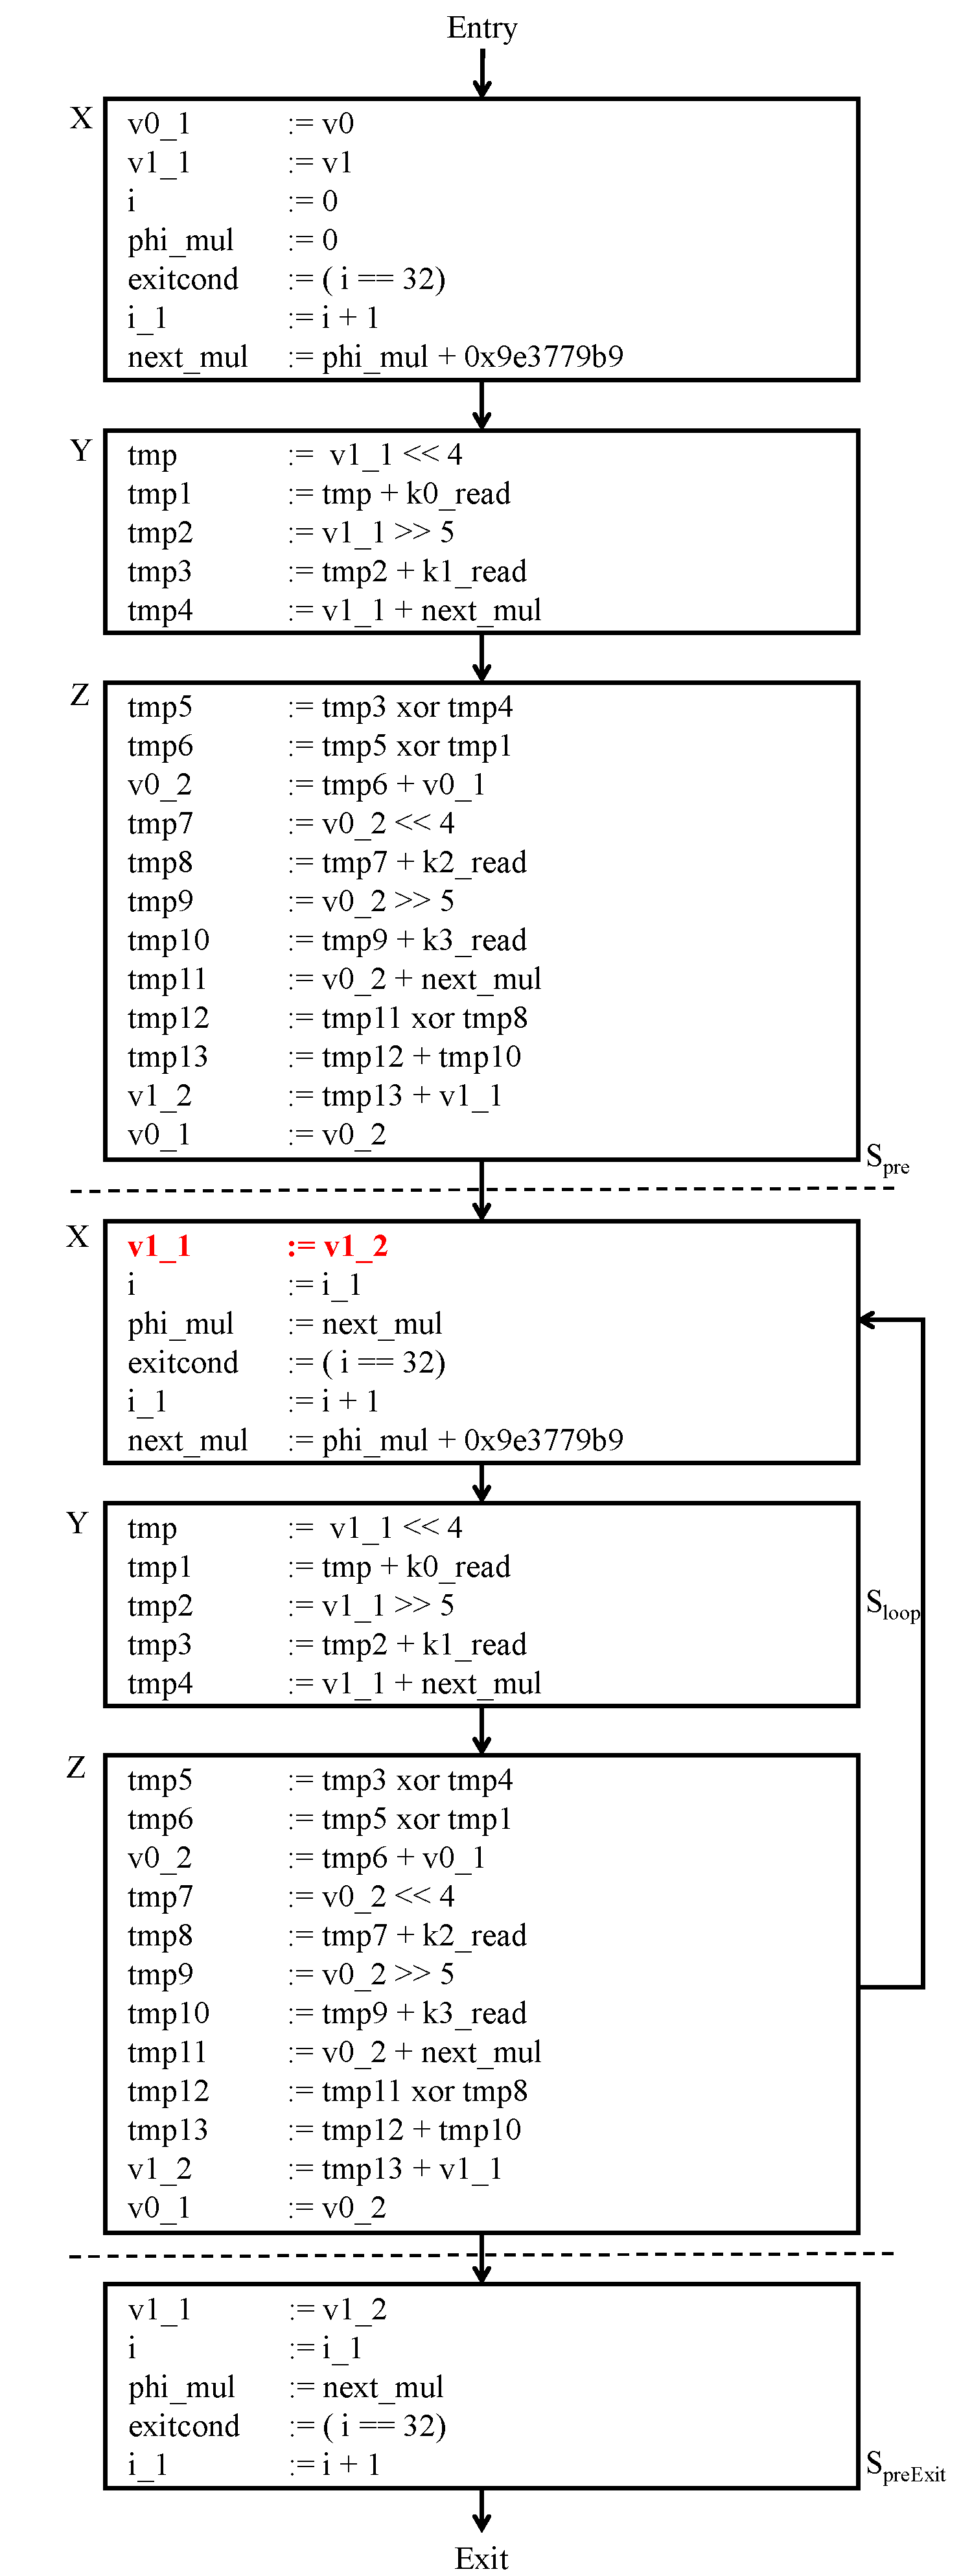
\includegraphics[height=8in]{fig-proposal/tea-after-data-propagation3}
\caption{TEA: After Data Propagation First Step for $v1\_1 := v1\_2$}
\label{fig:tea-after-data-propagation3}
\end{center}
\end{figure}

\begin{figure}[H]
\begin{center}
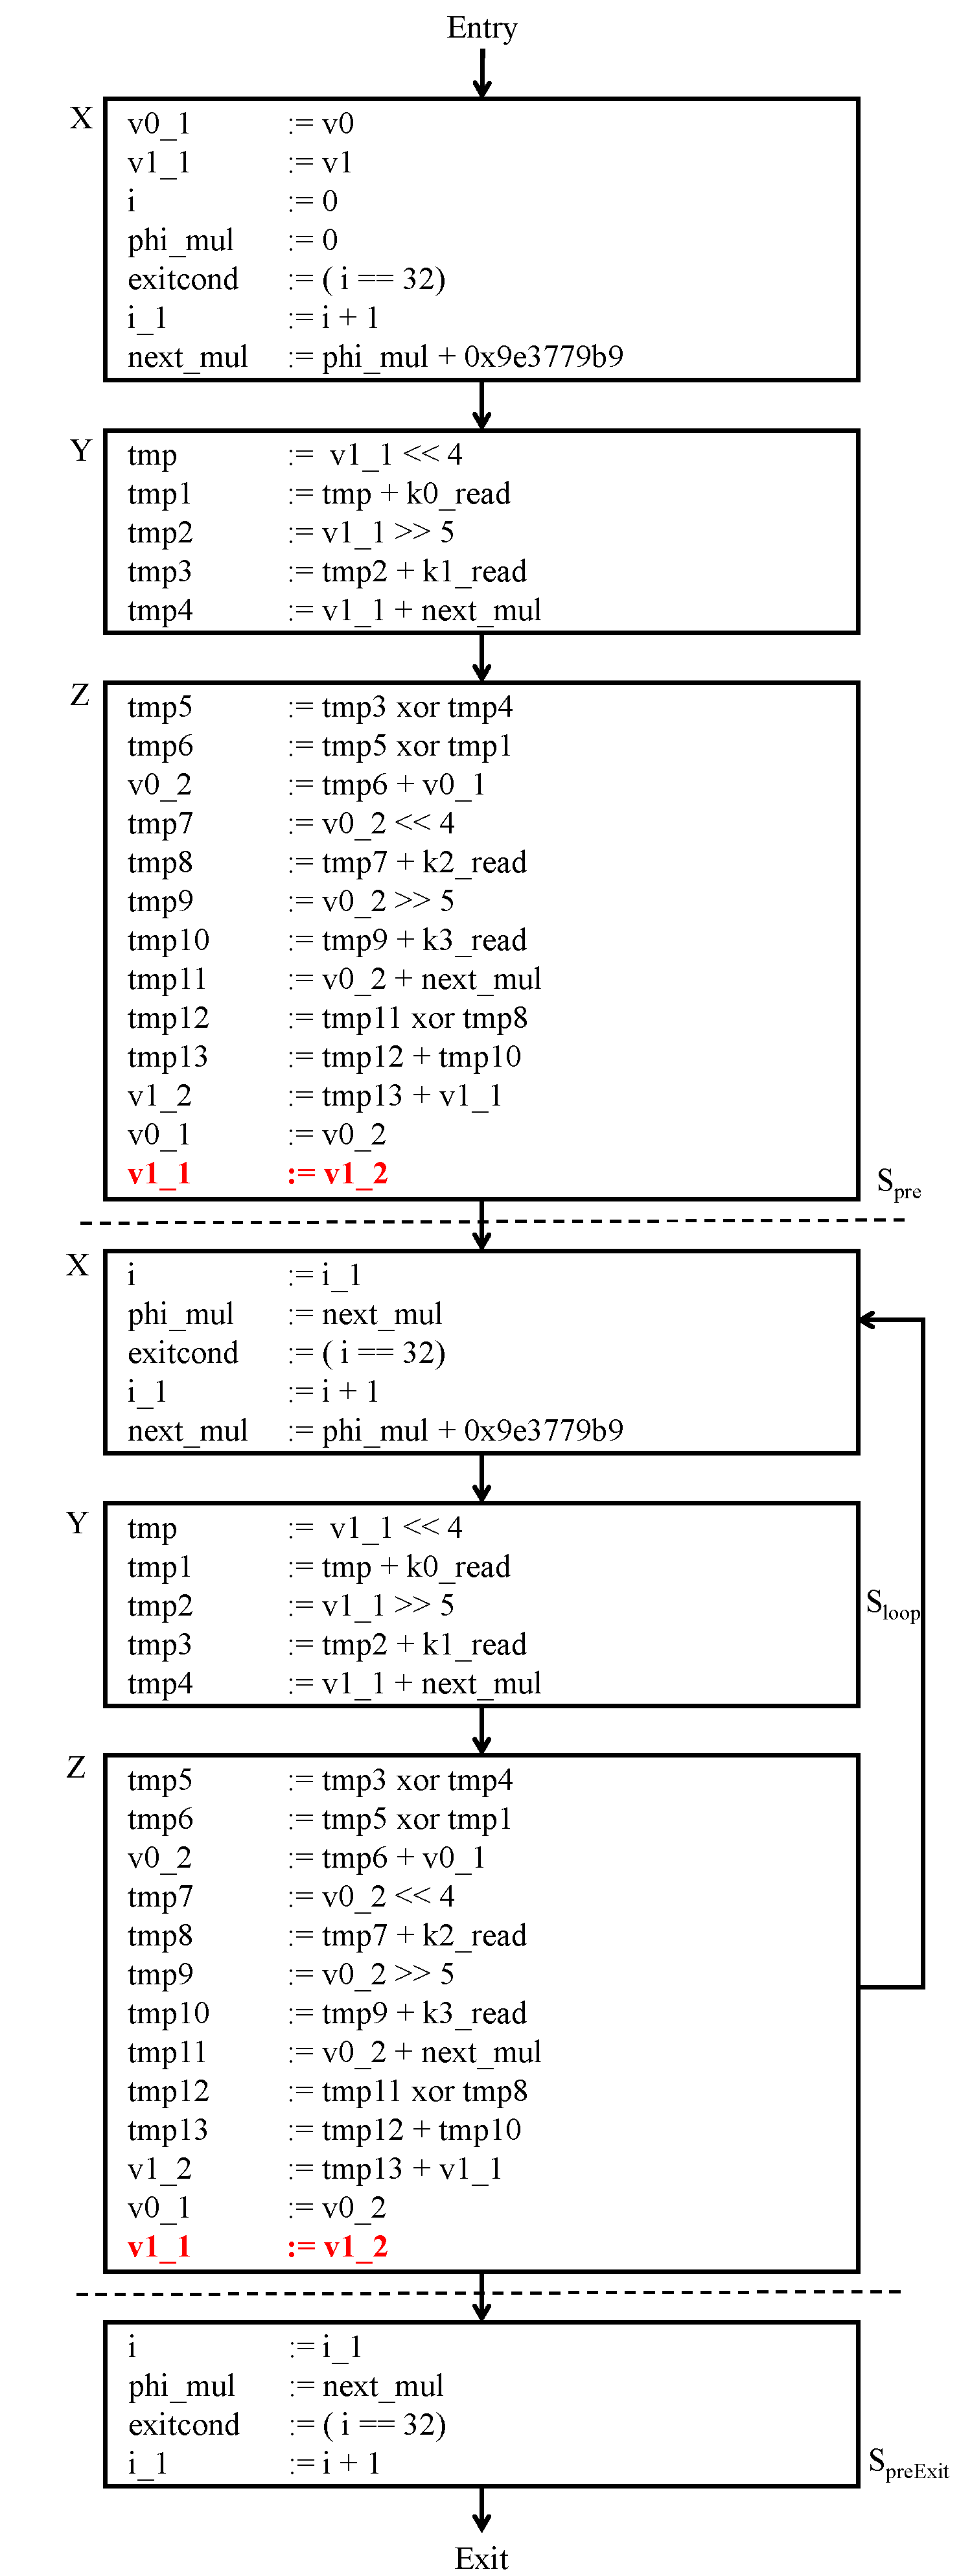
\includegraphics[height=8in]{fig-proposal/tea-after-data-propagation4}
\caption{TEA: After Data Propagation Second Step for $v1\_1 := v1\_2$}
\label{fig:tea-after-data-propagation4}
\end{center}
\end{figure}

After we have removed the potential WAR hazards which can stall the pipeline, we need to remove the RAW hazards as well.
We check the variables which can cause data hazards by measuring the read and write distance between variables 
and compare it to pipeline interval. For example, in Figure~\ref{fig:tea-after-data-propagation4}, we write $next\_mul$ 
in $X$ while we read $next\_mul$ in both $Y$ and $Z$. 
If we overlap the iterations as it is, then the $X$ of second iteration occurs before $Z$ of first iteration and we overwrite the value in 
$X$ before $Z$ has a chance to read it. Note that we know this as our algorithm calculates the longest read and write distance of every variable 
in an iteration. Here the distance for $next\_mul$ is 2 scheduling steps, while the pipeline interval is 1. So, we know that this
variable will cause a hazard when we pipeline. For all other variables, the distance is either 1 or 0 which is less than the pipeline interval so we know that they are
safe. 

We store the value of the variable in temporary variables called shadow registers, here we store the value in next\_reg, for second scheduling
step, we store in next\_reg2 and we read from these shadow registers so that the original value is unaffected and can be read as required. The new CCDFG with 
temporary variables is shown in Figure~\ref{fig:tea-after-shadow-register}.

Now, we can overlap the iterations as shown in Figure~\ref{fig:tea-after-superstep-construction}. We call this step - superstep construction. 

Now, we need to add the branches back which is the final step of our algorithm. We first interchange the $S\_{preExit}$ with $P\_{post}$. Since we have already removed the potential data hazards, we know that we can apply interchange primitives to achieve this step as shown in Figure ~\ref{fig:tea-after-interchange-post-exit}. Then, we apply the branch primitive and put the branch back to get the final pipelined structure as shown in Figure~\ref{fig:tea-after-adding-branches}.
 

\begin{figure}[H]
\begin{center}
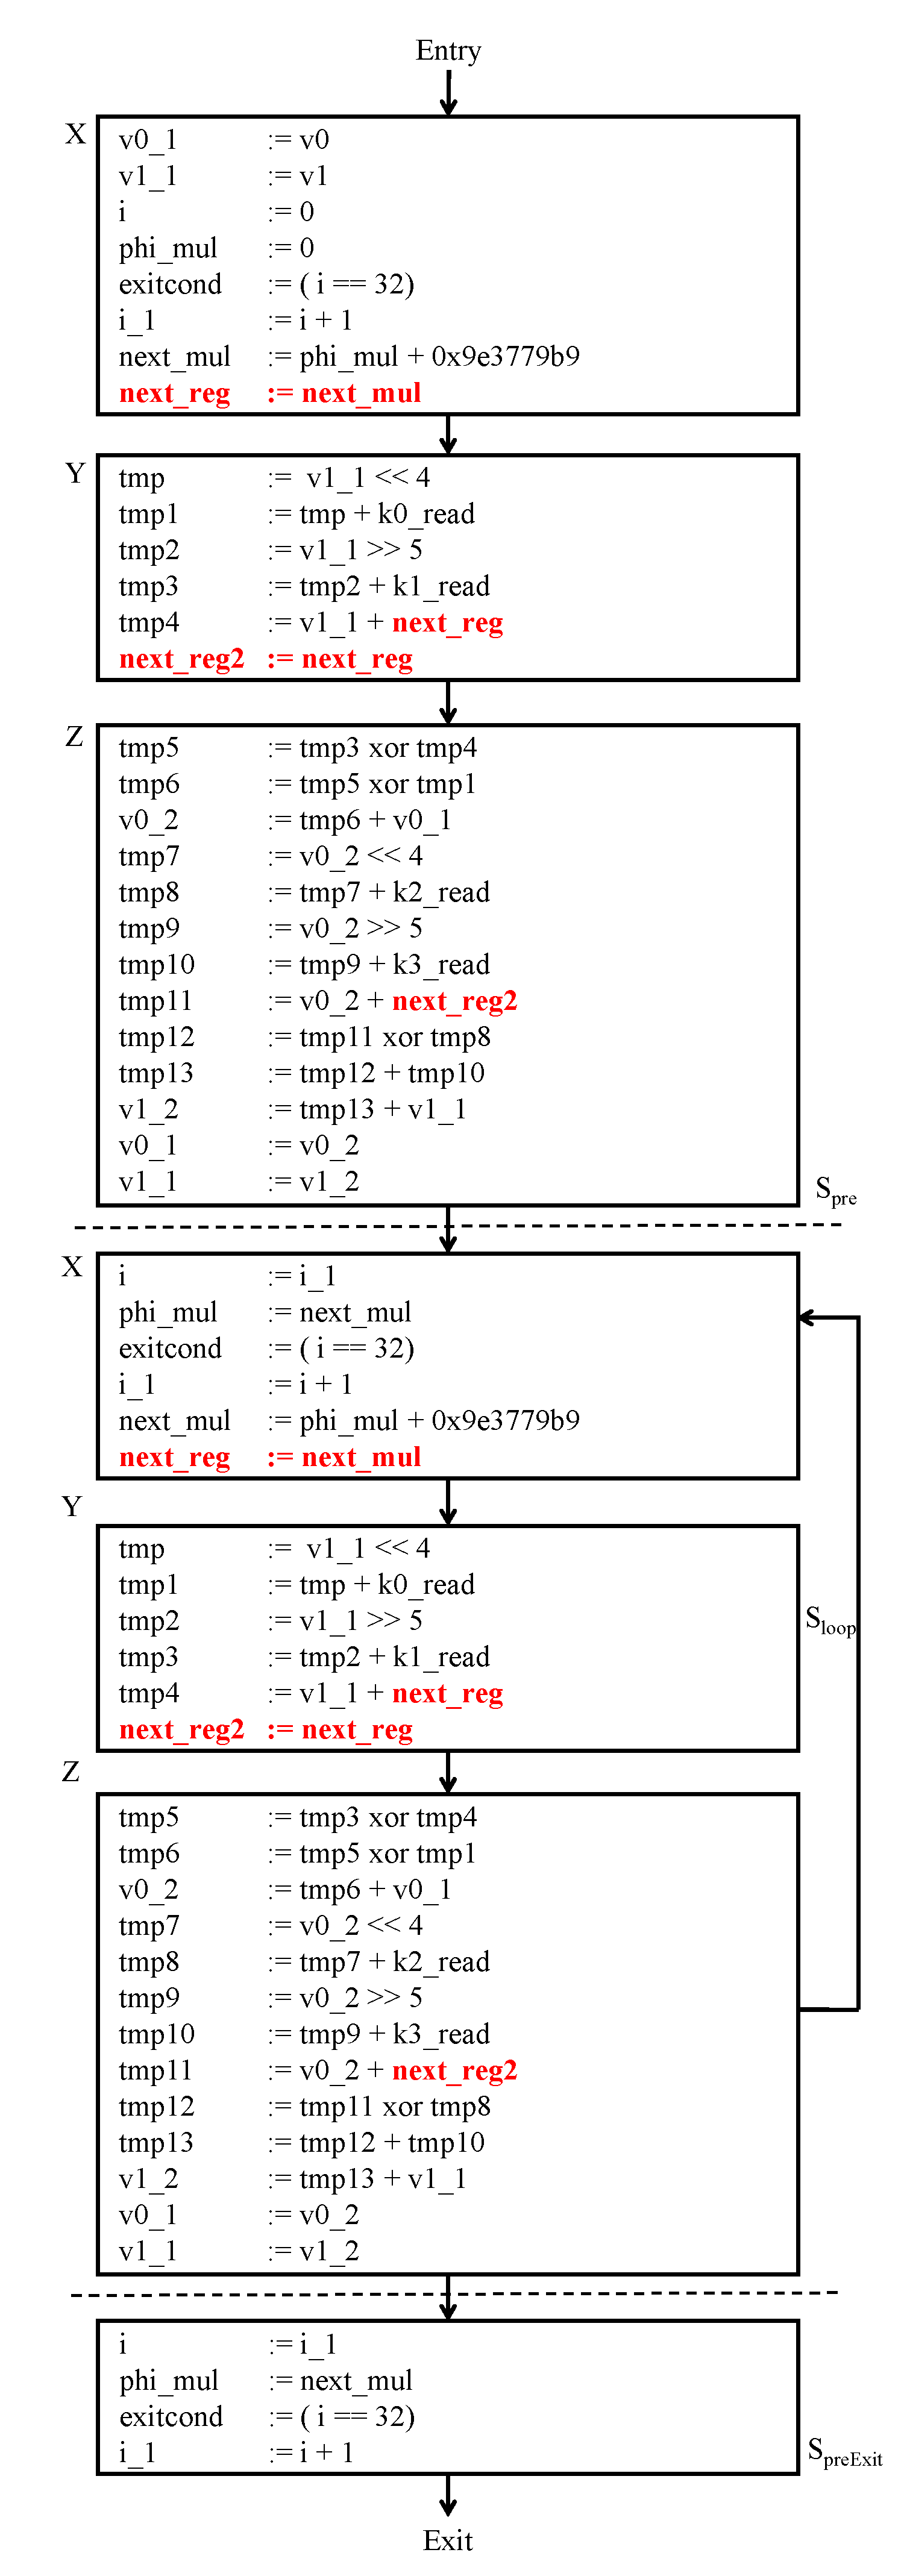
\includegraphics[height=8in]{fig-proposal/tea-after-shadow-reg}
\caption{TEA: After Adding Shadow Registers}
\label{fig:tea-after-shadow-register}
\end{center}
\end{figure}



\begin{figure}[H]
\begin{center}
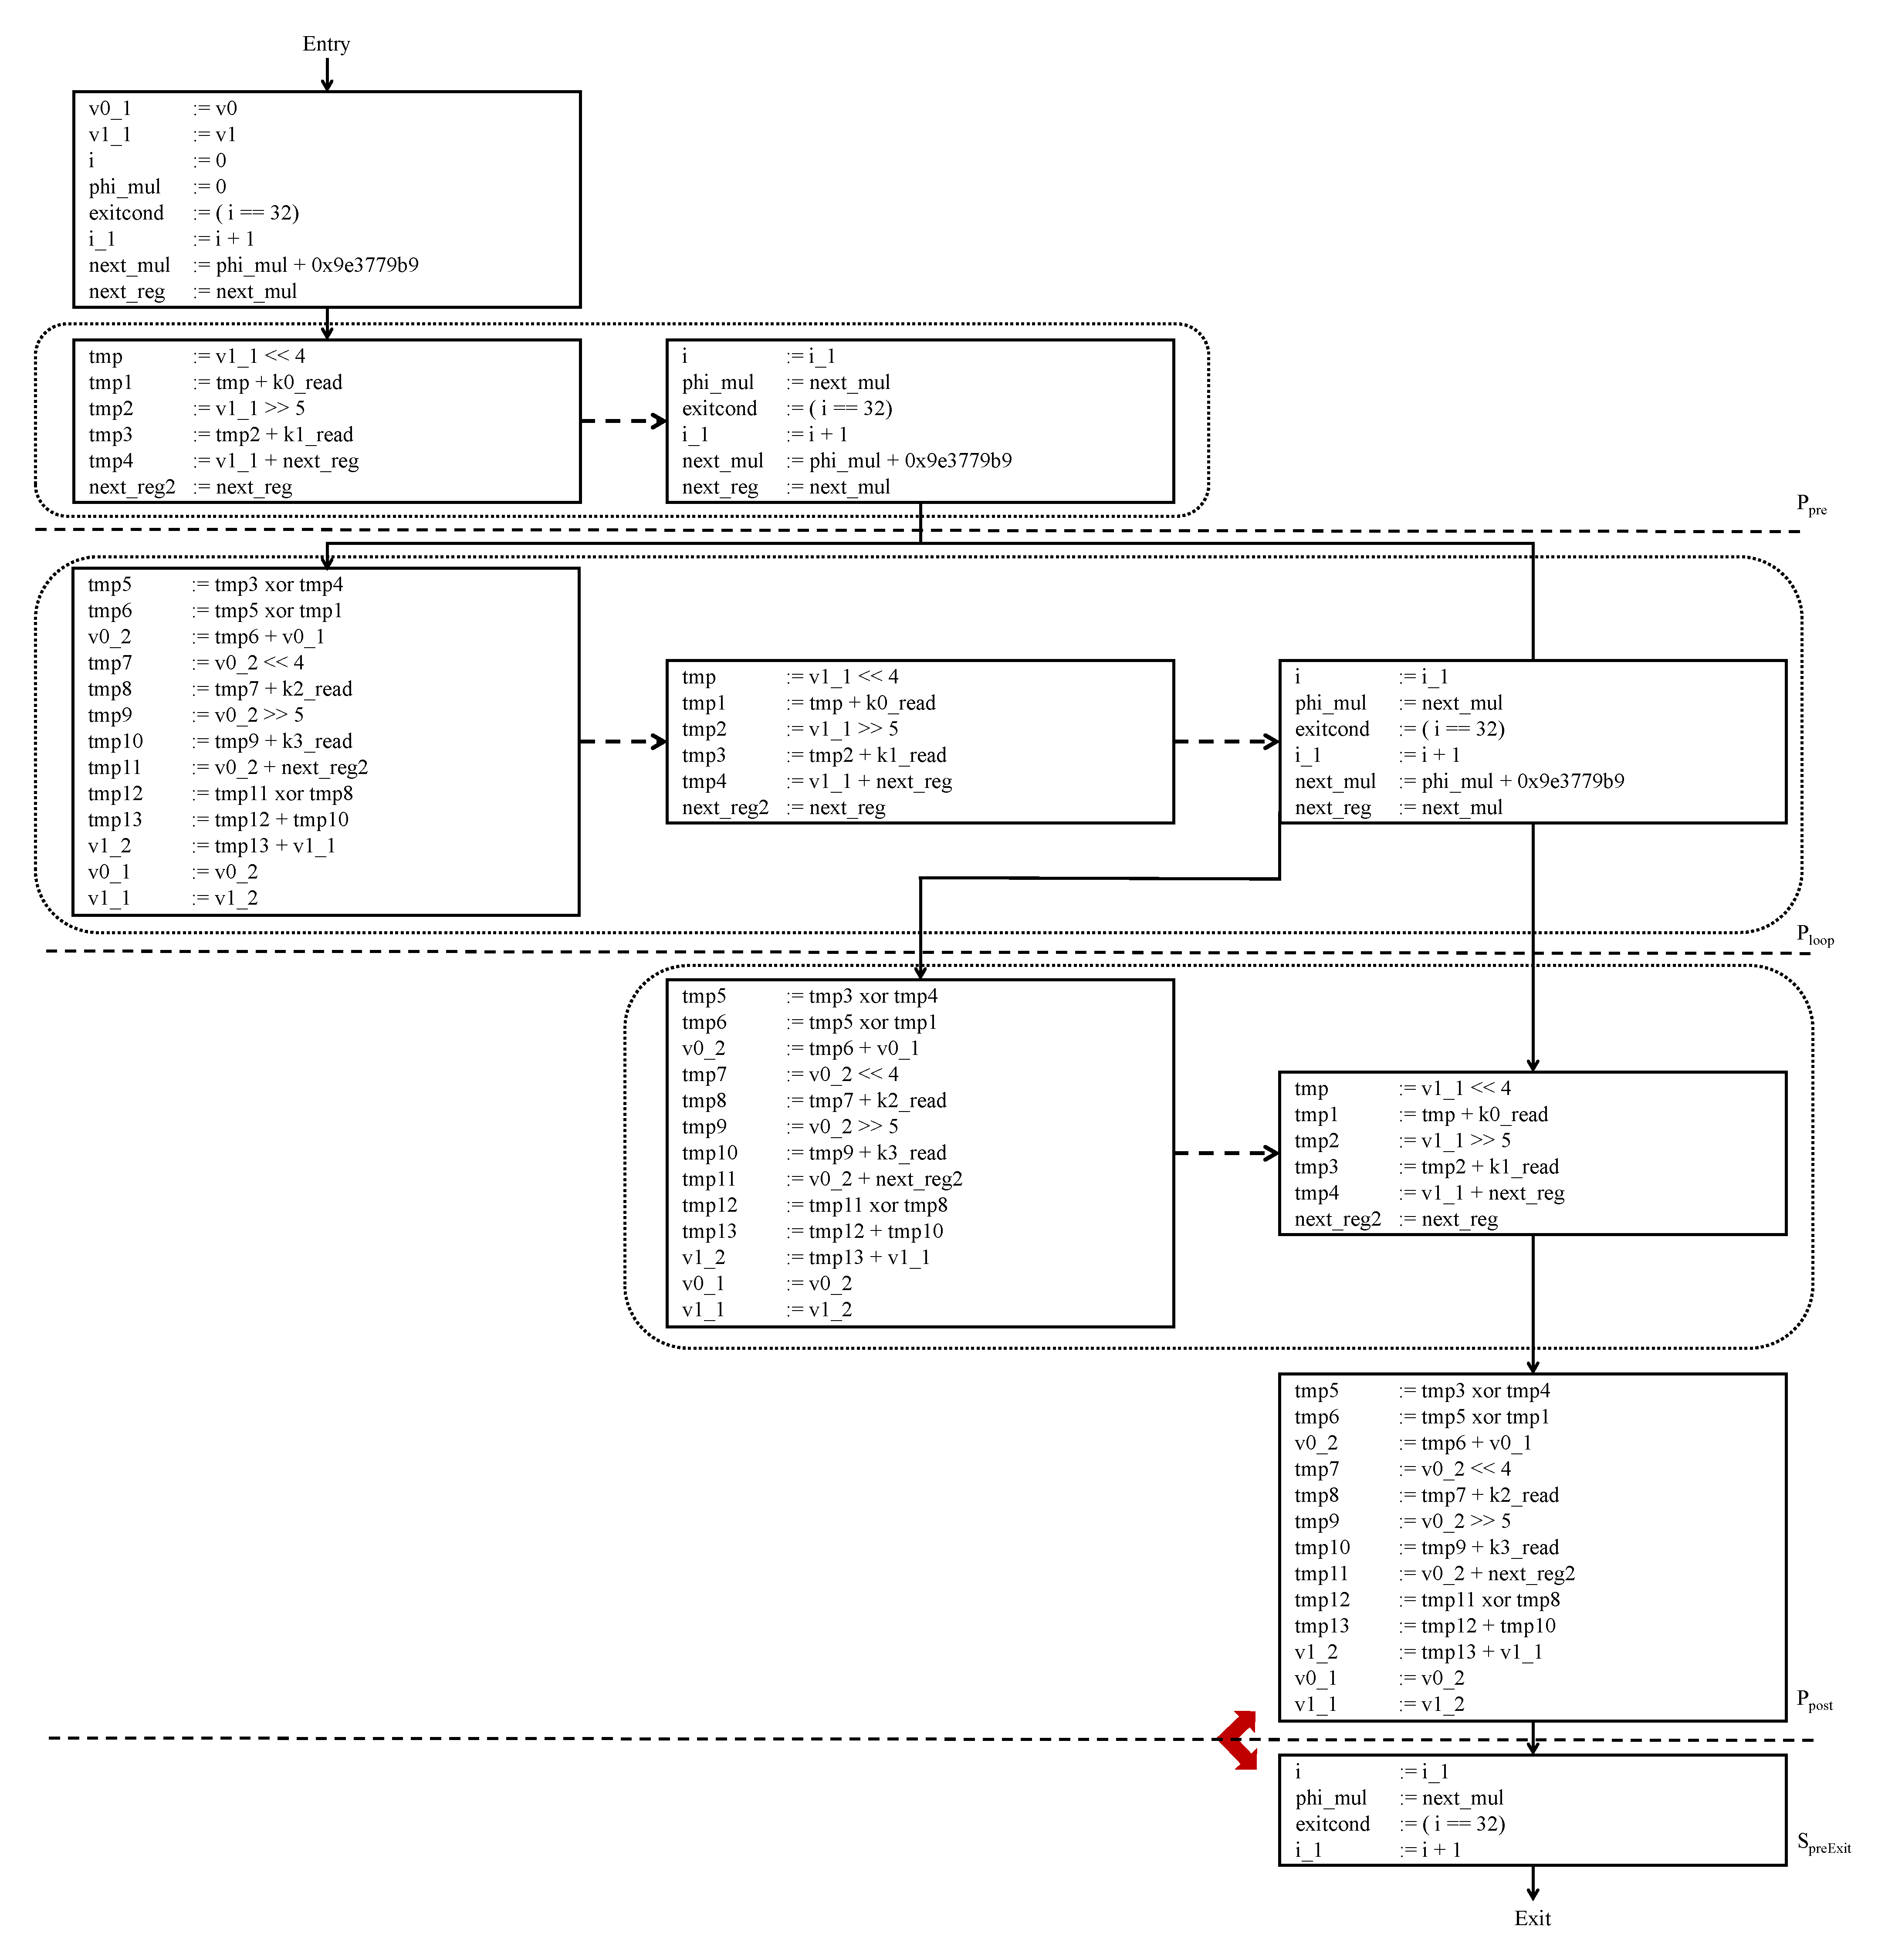
\includegraphics[width=5.5in]{fig-proposal/tea-after-superstep-construction}
\caption{TEA: After Superstep Construction}
\label{fig:tea-after-superstep-construction}
\end{center}
\end{figure}

\begin{figure}[H]
\begin{center}
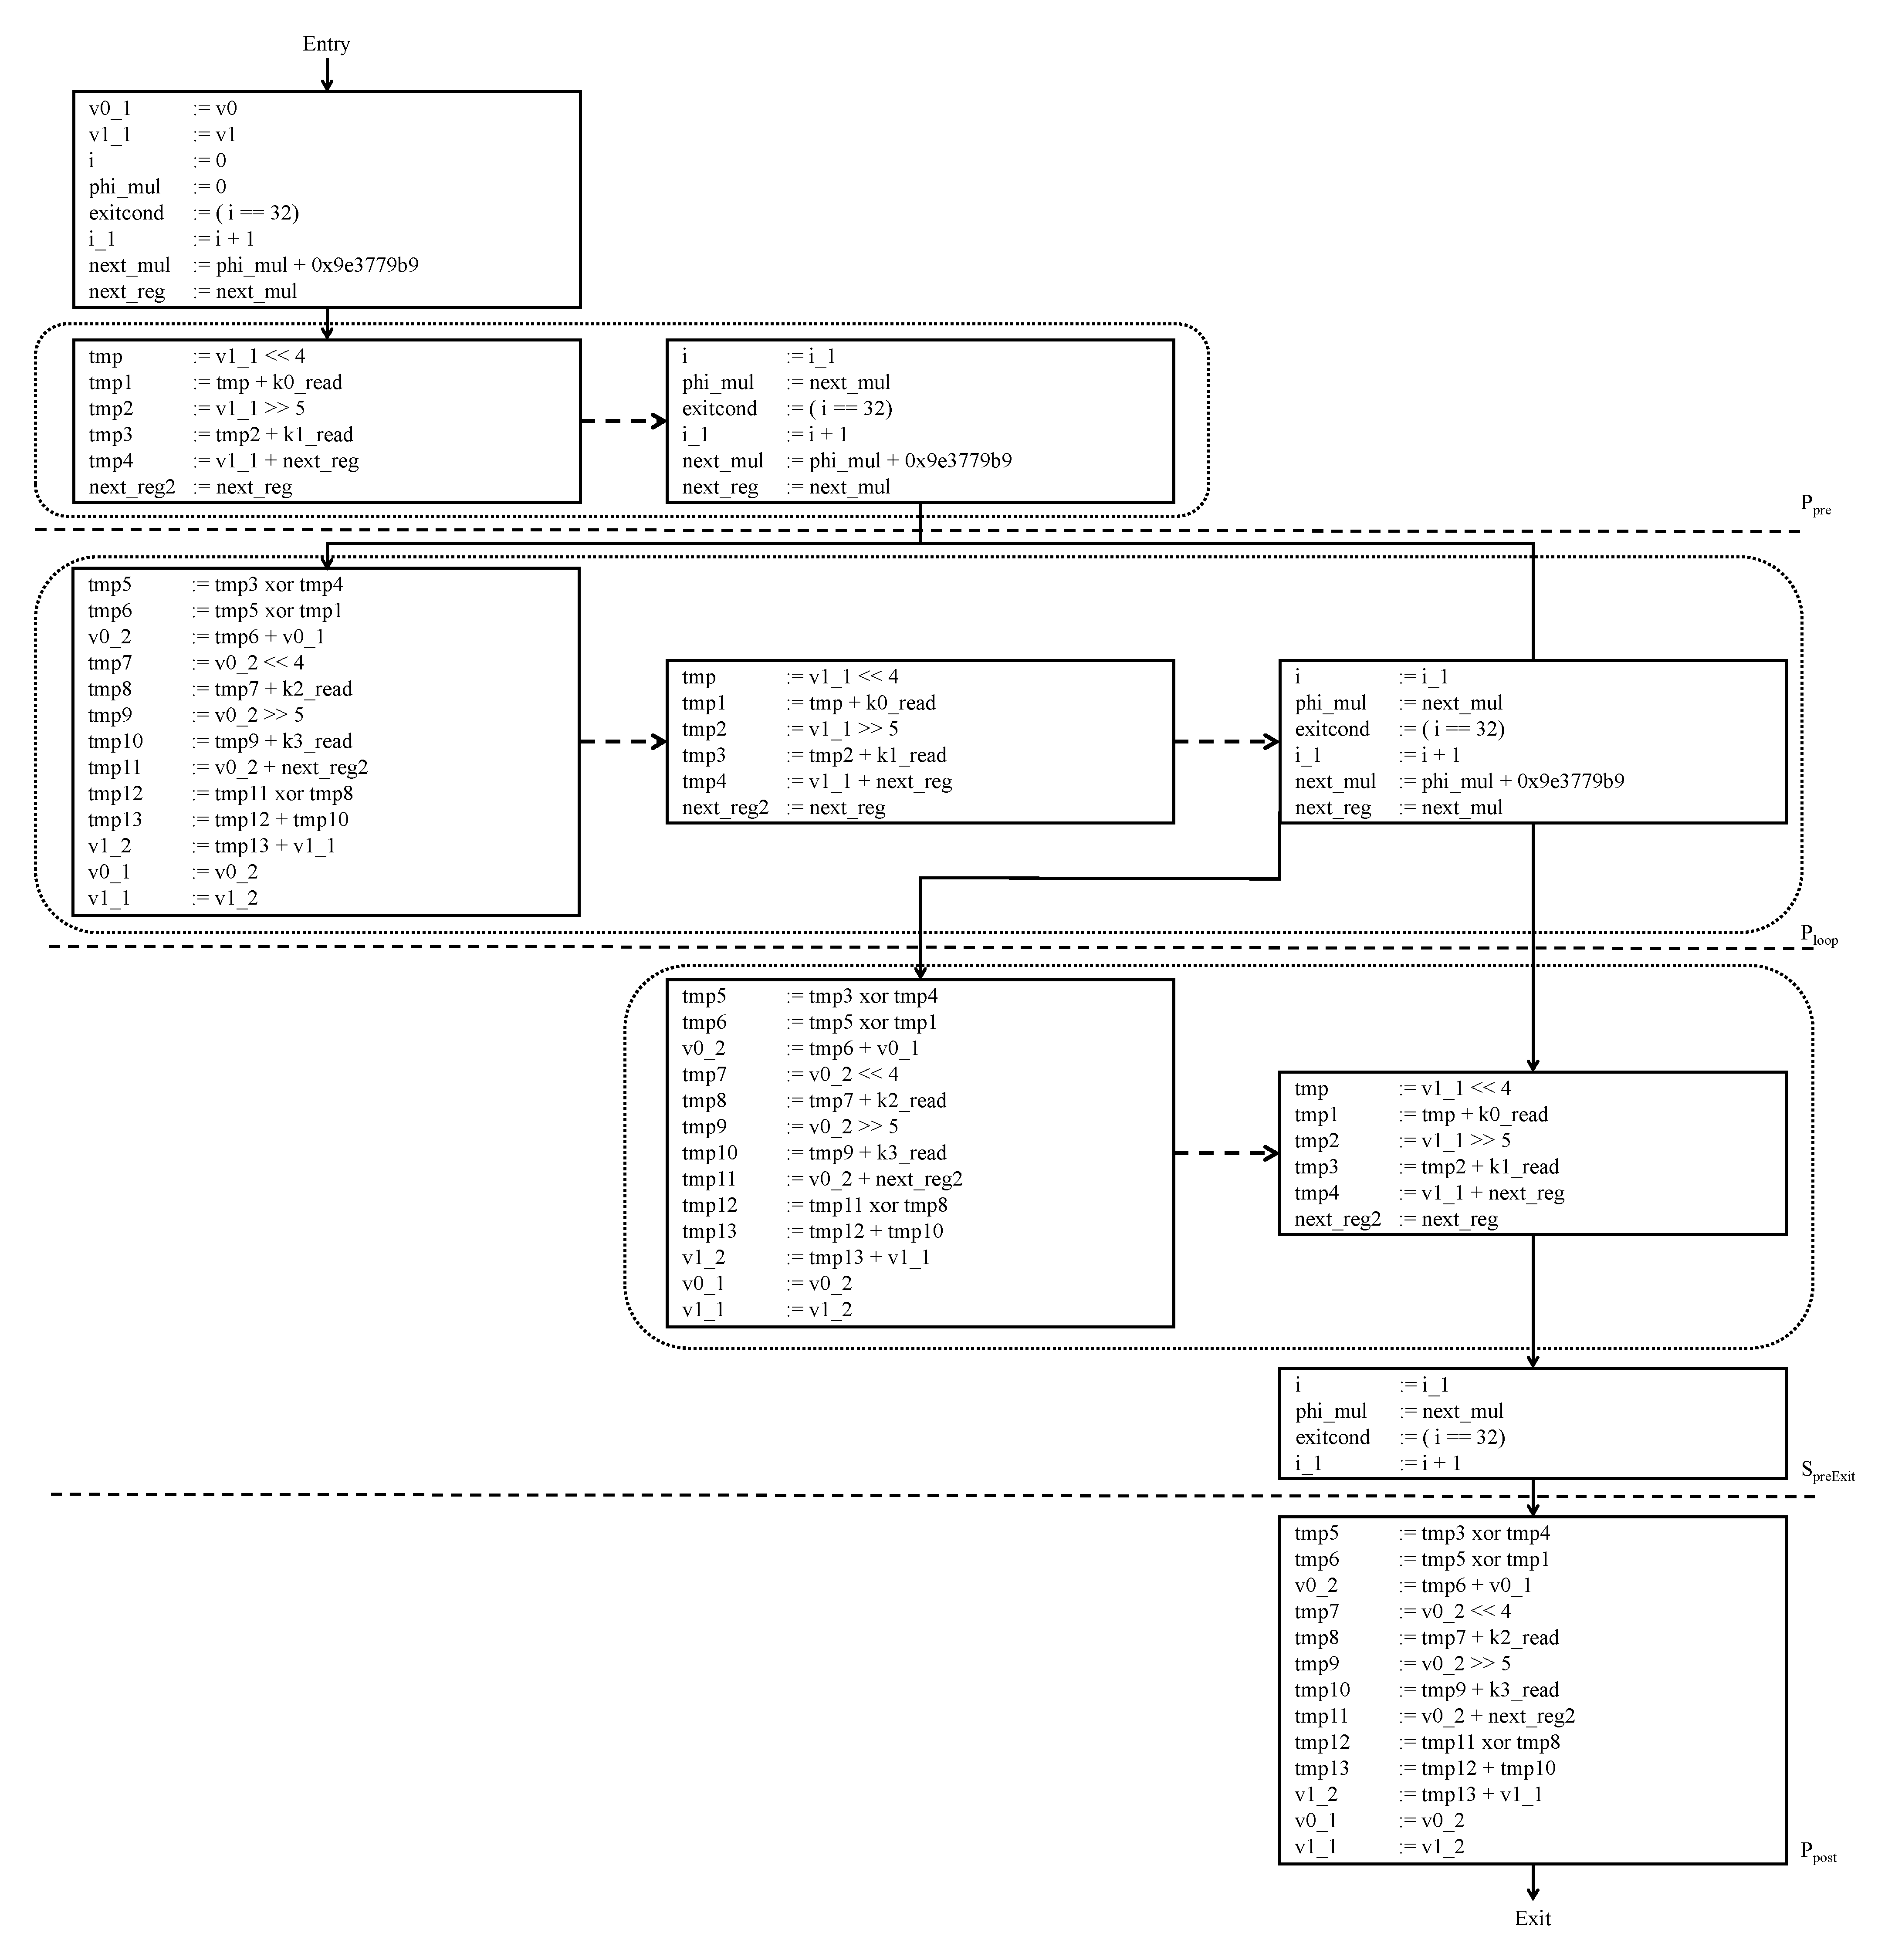
\includegraphics[width=5.5in]{fig-proposal/tea-after-interchange-pre-post}
\caption{TEA: After Interchanging Post with preExit}
\label{fig:tea-after-interchange-post-exit}
\end{center}
\end{figure}

\clearpage
\begin{sidewaysfigure}[t!]
\begin{center}
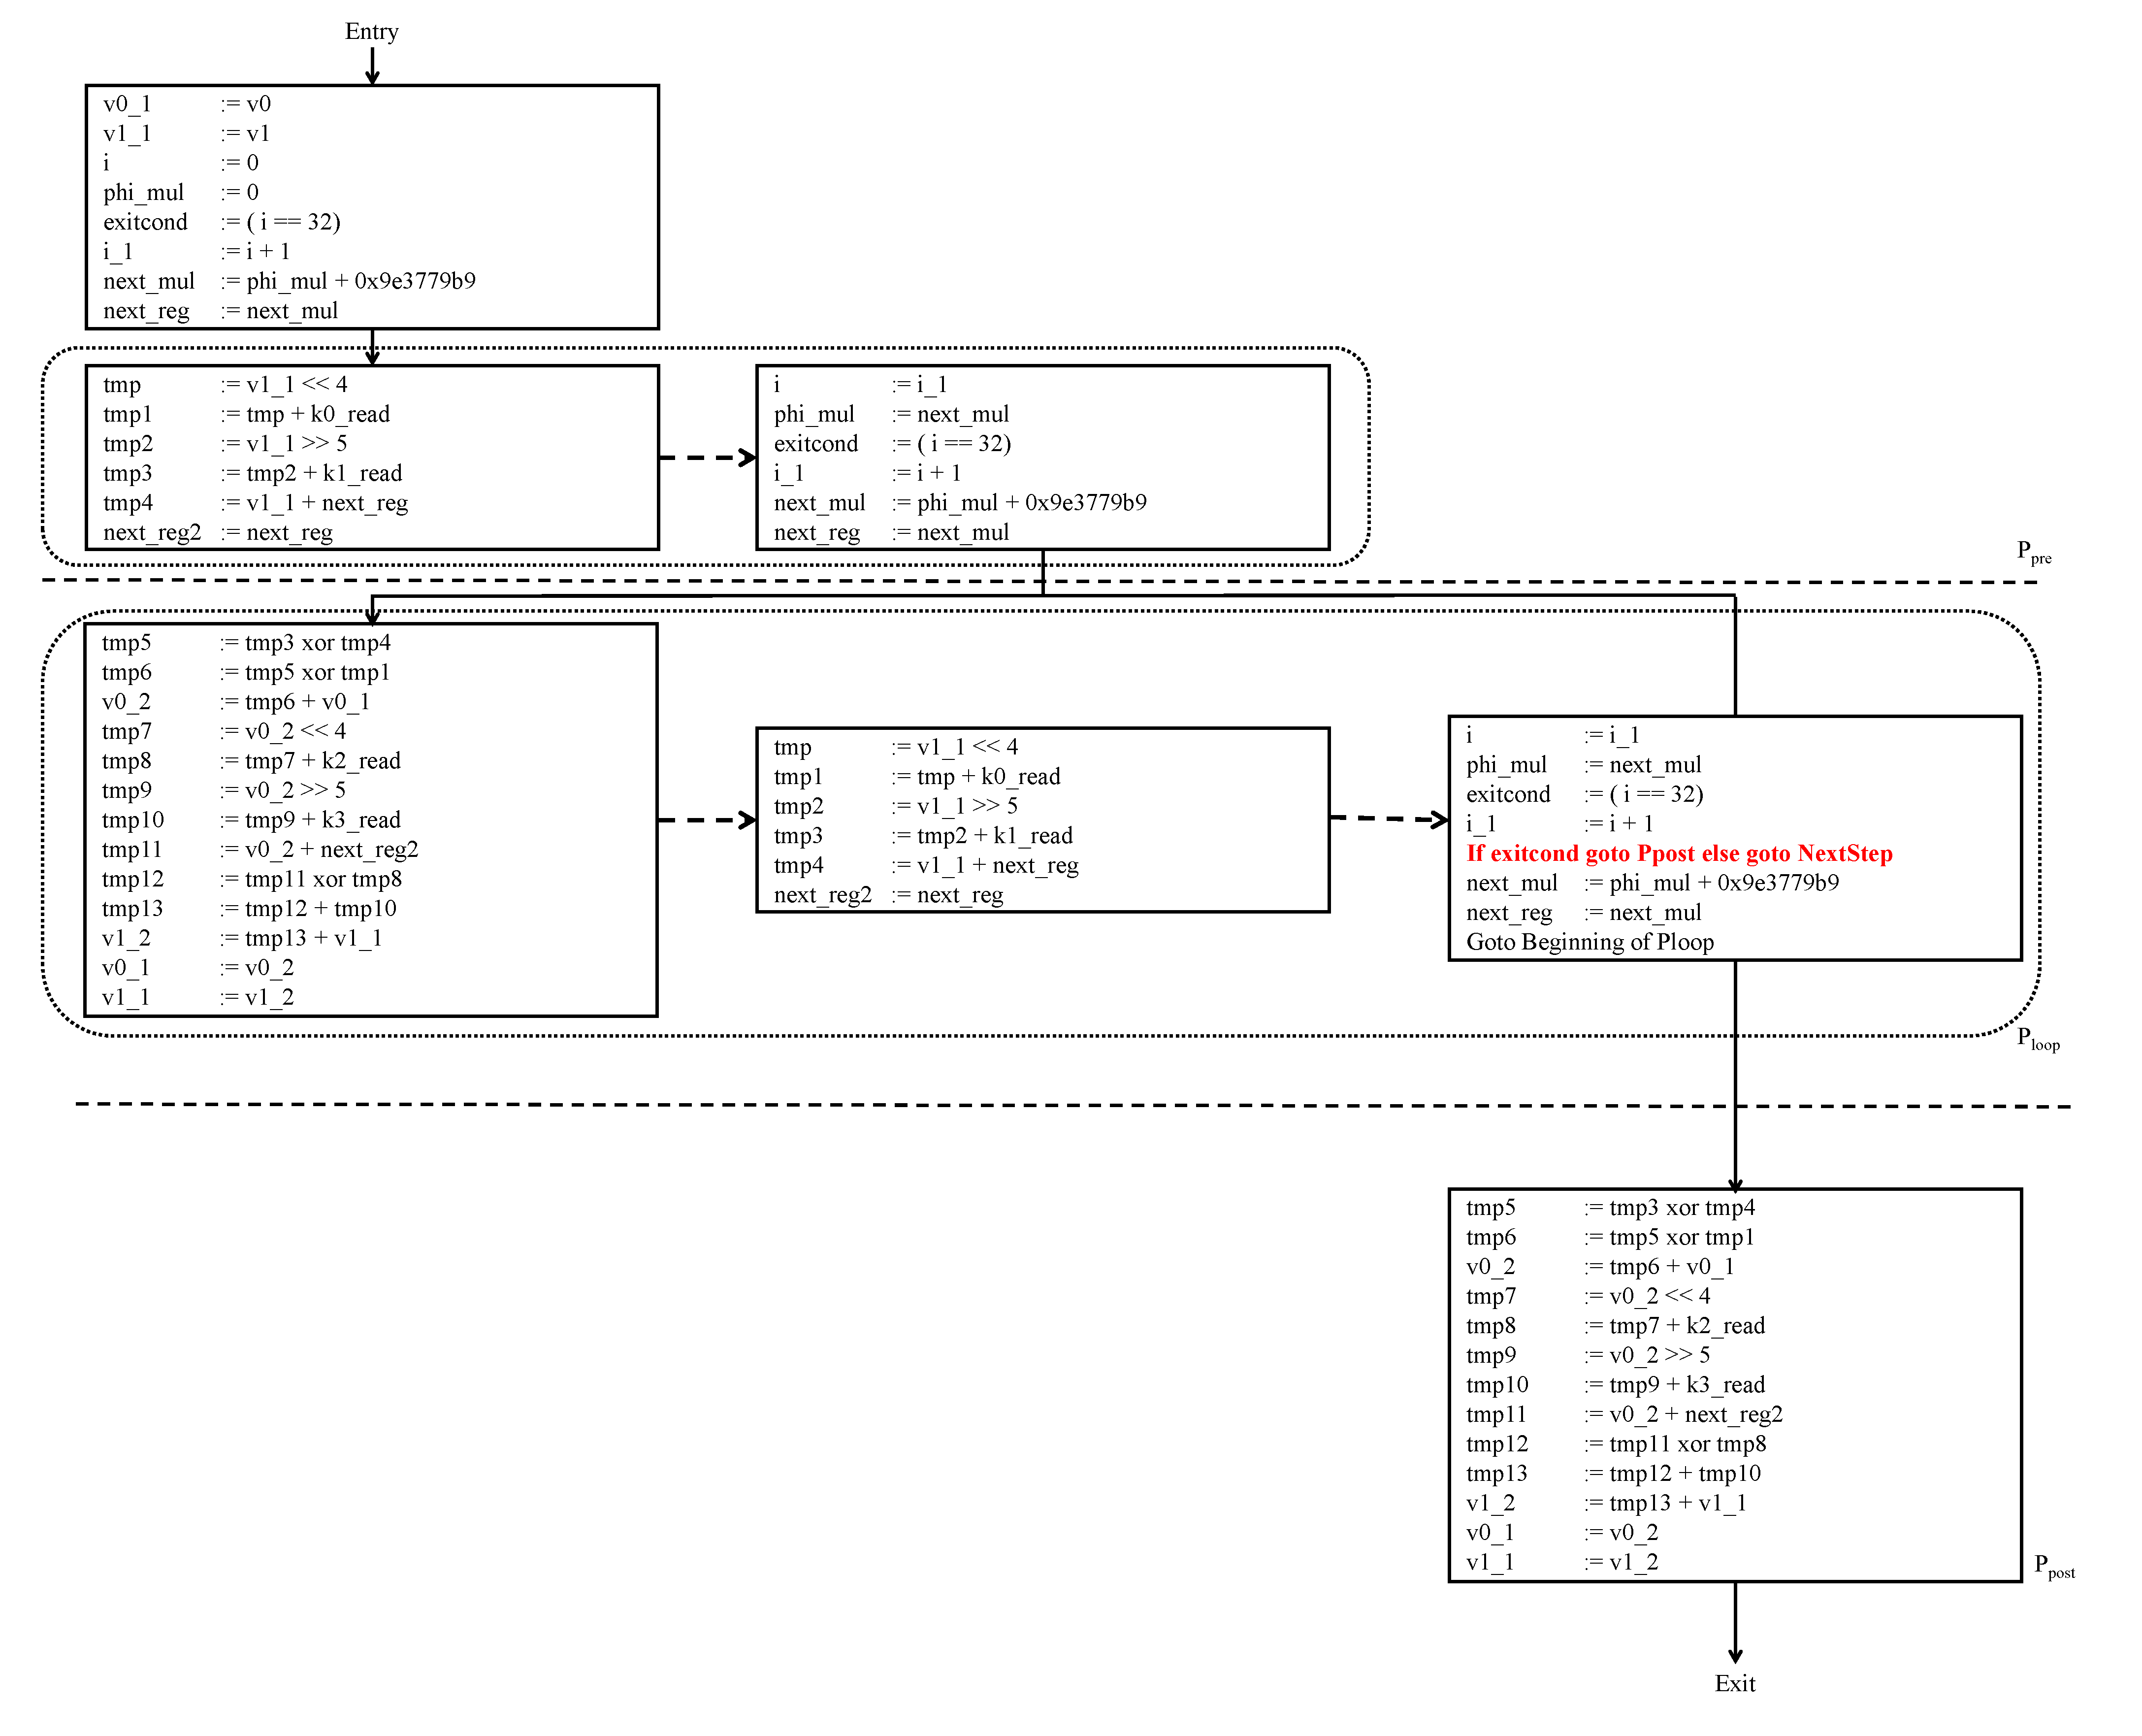
\includegraphics[height=5.5in]{fig-proposal/tea-after-adding-branches}
\end{center}
\caption{TEA: Pipelined CCDFG after adding branches back}
\label{fig:tea-after-adding-branches}
\end{sidewaysfigure}
\clearpage

As is evident from this example, we have a methodical way of dealing with data hazards and ensuring that we can get a smooth pipeline structure. 
We have shown that our approach works by testing it on industrial strength designs. The systematic approach to creating a pipelined structure has enabled 
us to succintly decompose our algorithm into certified primitives and thus certify the overall algorithm.





